% Version History
% 2020-10-27  	    Holger Graf
%                   Licence CC BY 4.0
%					Link: https://www.overleaf.com/latex/templates/thesis-template-microeconomics-at-fsu-jena/shqhkgcqtvsn
%					Accessed 18.01.2023
% 2023-02-01		Adapted by Ines Rieger
%					Licence CC BY 4.0
%					Lehrstuhl für Erklärbares Maschinelles Lernen
%					Universität Bamberg
% Please adapt this tex file for your thesis

\documentclass{xai-thesis}

\usepackage{graphicx}
\usepackage{setspace}
\usepackage{hyperref} % use \usepackage[hidelinks]{hyperref} to hide boxes
\usepackage[utf8]{inputenc} % depends on the font encoding that you are using
\usepackage[round]{natbib}
\usepackage{comment}

% SOURCE: https://github.com/goodfeli/dlbook_notation/blob/master/math_commands.tex
% Quote from github "We make them freely available for anyone to use."

\usepackage{amsmath,amsfonts,bm}


%%%%% NEW MATH DEFINITIONS %%%%%

% Mark sections of captions for referring to divisions of figures
\newcommand{\figleft}{{\em (Left)}}
\newcommand{\figcenter}{{\em (Center)}}
\newcommand{\figright}{{\em (Right)}}
\newcommand{\figtop}{{\em (Top)}}
\newcommand{\figbottom}{{\em (Bottom)}}
\newcommand{\captiona}{{\em (a)}}
\newcommand{\captionb}{{\em (b)}}
\newcommand{\captionc}{{\em (c)}}
\newcommand{\captiond}{{\em (d)}}

% Highlight a newly defined term
\newcommand{\newterm}[1]{{\bf #1}}


% Figure reference, lower-case.
\def\figref#1{figure~\ref{#1}}
% Figure reference, capital. For start of sentence
\def\Figref#1{Figure~\ref{#1}}
\def\twofigref#1#2{figures \ref{#1} and \ref{#2}}
\def\quadfigref#1#2#3#4{figures \ref{#1}, \ref{#2}, \ref{#3} and \ref{#4}}
% Section reference, lower-case.
\def\secref#1{section~\ref{#1}}
% Section reference, capital.
\def\Secref#1{Section~\ref{#1}}
% Reference to two sections.
\def\twosecrefs#1#2{sections \ref{#1} and \ref{#2}}
% Reference to three sections.
\def\secrefs#1#2#3{sections \ref{#1}, \ref{#2} and \ref{#3}}
% Reference to an equation, lower-case.
\def\eqref#1{equation~\ref{#1}}
% Reference to an equation, upper case
\def\Eqref#1{Equation~\ref{#1}}
% A raw reference to an equation---avoid using if possible
\def\plaineqref#1{\ref{#1}}
% Reference to a chapter, lower-case.
\def\chapref#1{chapter~\ref{#1}}
% Reference to an equation, upper case.
\def\Chapref#1{Chapter~\ref{#1}}
% Reference to a range of chapters
\def\rangechapref#1#2{chapters\ref{#1}--\ref{#2}}
% Reference to an algorithm, lower-case.
\def\algref#1{algorithm~\ref{#1}}
% Reference to an algorithm, upper case.
\def\Algref#1{Algorithm~\ref{#1}}
\def\twoalgref#1#2{algorithms \ref{#1} and \ref{#2}}
\def\Twoalgref#1#2{Algorithms \ref{#1} and \ref{#2}}
% Reference to a part, lower case
\def\partref#1{part~\ref{#1}}
% Reference to a part, upper case
\def\Partref#1{Part~\ref{#1}}
\def\twopartref#1#2{parts \ref{#1} and \ref{#2}}

\def\ceil#1{\lceil #1 \rceil}
\def\floor#1{\lfloor #1 \rfloor}
\def\1{\bm{1}}
\newcommand{\train}{\mathcal{D}}
\newcommand{\valid}{\mathcal{D_{\mathrm{valid}}}}
\newcommand{\test}{\mathcal{D_{\mathrm{test}}}}

\def\eps{{\epsilon}}


% Random variables
\def\reta{{\textnormal{$\eta$}}}
\def\ra{{\textnormal{a}}}
\def\rb{{\textnormal{b}}}
\def\rc{{\textnormal{c}}}
\def\rd{{\textnormal{d}}}
\def\re{{\textnormal{e}}}
\def\rf{{\textnormal{f}}}
\def\rg{{\textnormal{g}}}
\def\rh{{\textnormal{h}}}
\def\ri{{\textnormal{i}}}
\def\rj{{\textnormal{j}}}
\def\rk{{\textnormal{k}}}
\def\rl{{\textnormal{l}}}
% rm is already a command, just don't name any random variables m
\def\rn{{\textnormal{n}}}
\def\ro{{\textnormal{o}}}
\def\rp{{\textnormal{p}}}
\def\rq{{\textnormal{q}}}
\def\rr{{\textnormal{r}}}
\def\rs{{\textnormal{s}}}
\def\rt{{\textnormal{t}}}
\def\ru{{\textnormal{u}}}
\def\rv{{\textnormal{v}}}
\def\rw{{\textnormal{w}}}
\def\rx{{\textnormal{x}}}
\def\ry{{\textnormal{y}}}
\def\rz{{\textnormal{z}}}

% Random vectors
\def\rvepsilon{{\mathbf{\epsilon}}}
\def\rvtheta{{\mathbf{\theta}}}
\def\rva{{\mathbf{a}}}
\def\rvb{{\mathbf{b}}}
\def\rvc{{\mathbf{c}}}
\def\rvd{{\mathbf{d}}}
\def\rve{{\mathbf{e}}}
\def\rvf{{\mathbf{f}}}
\def\rvg{{\mathbf{g}}}
\def\rvh{{\mathbf{h}}}
\def\rvu{{\mathbf{i}}}
\def\rvj{{\mathbf{j}}}
\def\rvk{{\mathbf{k}}}
\def\rvl{{\mathbf{l}}}
\def\rvm{{\mathbf{m}}}
\def\rvn{{\mathbf{n}}}
\def\rvo{{\mathbf{o}}}
\def\rvp{{\mathbf{p}}}
\def\rvq{{\mathbf{q}}}
\def\rvr{{\mathbf{r}}}
\def\rvs{{\mathbf{s}}}
\def\rvt{{\mathbf{t}}}
\def\rvu{{\mathbf{u}}}
\def\rvv{{\mathbf{v}}}
\def\rvw{{\mathbf{w}}}
\def\rvx{{\mathbf{x}}}
\def\rvy{{\mathbf{y}}}
\def\rvz{{\mathbf{z}}}

% Elements of random vectors
\def\erva{{\textnormal{a}}}
\def\ervb{{\textnormal{b}}}
\def\ervc{{\textnormal{c}}}
\def\ervd{{\textnormal{d}}}
\def\erve{{\textnormal{e}}}
\def\ervf{{\textnormal{f}}}
\def\ervg{{\textnormal{g}}}
\def\ervh{{\textnormal{h}}}
\def\ervi{{\textnormal{i}}}
\def\ervj{{\textnormal{j}}}
\def\ervk{{\textnormal{k}}}
\def\ervl{{\textnormal{l}}}
\def\ervm{{\textnormal{m}}}
\def\ervn{{\textnormal{n}}}
\def\ervo{{\textnormal{o}}}
\def\ervp{{\textnormal{p}}}
\def\ervq{{\textnormal{q}}}
\def\ervr{{\textnormal{r}}}
\def\ervs{{\textnormal{s}}}
\def\ervt{{\textnormal{t}}}
\def\ervu{{\textnormal{u}}}
\def\ervv{{\textnormal{v}}}
\def\ervw{{\textnormal{w}}}
\def\ervx{{\textnormal{x}}}
\def\ervy{{\textnormal{y}}}
\def\ervz{{\textnormal{z}}}

% Random matrices
\def\rmA{{\mathbf{A}}}
\def\rmB{{\mathbf{B}}}
\def\rmC{{\mathbf{C}}}
\def\rmD{{\mathbf{D}}}
\def\rmE{{\mathbf{E}}}
\def\rmF{{\mathbf{F}}}
\def\rmG{{\mathbf{G}}}
\def\rmH{{\mathbf{H}}}
\def\rmI{{\mathbf{I}}}
\def\rmJ{{\mathbf{J}}}
\def\rmK{{\mathbf{K}}}
\def\rmL{{\mathbf{L}}}
\def\rmM{{\mathbf{M}}}
\def\rmN{{\mathbf{N}}}
\def\rmO{{\mathbf{O}}}
\def\rmP{{\mathbf{P}}}
\def\rmQ{{\mathbf{Q}}}
\def\rmR{{\mathbf{R}}}
\def\rmS{{\mathbf{S}}}
\def\rmT{{\mathbf{T}}}
\def\rmU{{\mathbf{U}}}
\def\rmV{{\mathbf{V}}}
\def\rmW{{\mathbf{W}}}
\def\rmX{{\mathbf{X}}}
\def\rmY{{\mathbf{Y}}}
\def\rmZ{{\mathbf{Z}}}

% Elements of random matrices
\def\ermA{{\textnormal{A}}}
\def\ermB{{\textnormal{B}}}
\def\ermC{{\textnormal{C}}}
\def\ermD{{\textnormal{D}}}
\def\ermE{{\textnormal{E}}}
\def\ermF{{\textnormal{F}}}
\def\ermG{{\textnormal{G}}}
\def\ermH{{\textnormal{H}}}
\def\ermI{{\textnormal{I}}}
\def\ermJ{{\textnormal{J}}}
\def\ermK{{\textnormal{K}}}
\def\ermL{{\textnormal{L}}}
\def\ermM{{\textnormal{M}}}
\def\ermN{{\textnormal{N}}}
\def\ermO{{\textnormal{O}}}
\def\ermP{{\textnormal{P}}}
\def\ermQ{{\textnormal{Q}}}
\def\ermR{{\textnormal{R}}}
\def\ermS{{\textnormal{S}}}
\def\ermT{{\textnormal{T}}}
\def\ermU{{\textnormal{U}}}
\def\ermV{{\textnormal{V}}}
\def\ermW{{\textnormal{W}}}
\def\ermX{{\textnormal{X}}}
\def\ermY{{\textnormal{Y}}}
\def\ermZ{{\textnormal{Z}}}

% Vectors
\def\vzero{{\bm{0}}}
\def\vone{{\bm{1}}}
\def\vmu{{\bm{\mu}}}
\def\vtheta{{\bm{\theta}}}
\def\va{{\bm{a}}}
\def\vb{{\bm{b}}}
\def\vc{{\bm{c}}}
\def\vd{{\bm{d}}}
\def\ve{{\bm{e}}}
\def\vf{{\bm{f}}}
\def\vg{{\bm{g}}}
\def\vh{{\bm{h}}}
\def\vi{{\bm{i}}}
\def\vj{{\bm{j}}}
\def\vk{{\bm{k}}}
\def\vl{{\bm{l}}}
\def\vm{{\bm{m}}}
\def\vn{{\bm{n}}}
\def\vo{{\bm{o}}}
\def\vp{{\bm{p}}}
\def\vq{{\bm{q}}}
\def\vr{{\bm{r}}}
\def\vs{{\bm{s}}}
\def\vt{{\bm{t}}}
\def\vu{{\bm{u}}}
\def\vv{{\bm{v}}}
\def\vw{{\bm{w}}}
\def\vx{{\bm{x}}}
\def\vy{{\bm{y}}}
\def\vz{{\bm{z}}}

% Elements of vectors
\def\evalpha{{\alpha}}
\def\evbeta{{\beta}}
\def\evepsilon{{\epsilon}}
\def\evlambda{{\lambda}}
\def\evomega{{\omega}}
\def\evmu{{\mu}}
\def\evpsi{{\psi}}
\def\evsigma{{\sigma}}
\def\evtheta{{\theta}}
\def\eva{{a}}
\def\evb{{b}}
\def\evc{{c}}
\def\evd{{d}}
\def\eve{{e}}
\def\evf{{f}}
\def\evg{{g}}
\def\evh{{h}}
\def\evi{{i}}
\def\evj{{j}}
\def\evk{{k}}
\def\evl{{l}}
\def\evm{{m}}
\def\evn{{n}}
\def\evo{{o}}
\def\evp{{p}}
\def\evq{{q}}
\def\evr{{r}}
\def\evs{{s}}
\def\evt{{t}}
\def\evu{{u}}
\def\evv{{v}}
\def\evw{{w}}
\def\evx{{x}}
\def\evy{{y}}
\def\evz{{z}}

% Matrix
\def\mA{{\bm{A}}}
\def\mB{{\bm{B}}}
\def\mC{{\bm{C}}}
\def\mD{{\bm{D}}}
\def\mE{{\bm{E}}}
\def\mF{{\bm{F}}}
\def\mG{{\bm{G}}}
\def\mH{{\bm{H}}}
\def\mI{{\bm{I}}}
\def\mJ{{\bm{J}}}
\def\mK{{\bm{K}}}
\def\mL{{\bm{L}}}
\def\mM{{\bm{M}}}
\def\mN{{\bm{N}}}
\def\mO{{\bm{O}}}
\def\mP{{\bm{P}}}
\def\mQ{{\bm{Q}}}
\def\mR{{\bm{R}}}
\def\mS{{\bm{S}}}
\def\mT{{\bm{T}}}
\def\mU{{\bm{U}}}
\def\mV{{\bm{V}}}
\def\mW{{\bm{W}}}
\def\mX{{\bm{X}}}
\def\mY{{\bm{Y}}}
\def\mZ{{\bm{Z}}}
\def\mBeta{{\bm{\beta}}}
\def\mPhi{{\bm{\Phi}}}
\def\mLambda{{\bm{\Lambda}}}
\def\mSigma{{\bm{\Sigma}}}

% Tensor
\DeclareMathAlphabet{\mathsfit}{\encodingdefault}{\sfdefault}{m}{sl}
\SetMathAlphabet{\mathsfit}{bold}{\encodingdefault}{\sfdefault}{bx}{n}
\newcommand{\tens}[1]{\bm{\mathsfit{#1}}}
\def\tA{{\tens{A}}}
\def\tB{{\tens{B}}}
\def\tC{{\tens{C}}}
\def\tD{{\tens{D}}}
\def\tE{{\tens{E}}}
\def\tF{{\tens{F}}}
\def\tG{{\tens{G}}}
\def\tH{{\tens{H}}}
\def\tI{{\tens{I}}}
\def\tJ{{\tens{J}}}
\def\tK{{\tens{K}}}
\def\tL{{\tens{L}}}
\def\tM{{\tens{M}}}
\def\tN{{\tens{N}}}
\def\tO{{\tens{O}}}
\def\tP{{\tens{P}}}
\def\tQ{{\tens{Q}}}
\def\tR{{\tens{R}}}
\def\tS{{\tens{S}}}
\def\tT{{\tens{T}}}
\def\tU{{\tens{U}}}
\def\tV{{\tens{V}}}
\def\tW{{\tens{W}}}
\def\tX{{\tens{X}}}
\def\tY{{\tens{Y}}}
\def\tZ{{\tens{Z}}}


% Graph
\def\gA{{\mathcal{A}}}
\def\gB{{\mathcal{B}}}
\def\gC{{\mathcal{C}}}
\def\gD{{\mathcal{D}}}
\def\gE{{\mathcal{E}}}
\def\gF{{\mathcal{F}}}
\def\gG{{\mathcal{G}}}
\def\gH{{\mathcal{H}}}
\def\gI{{\mathcal{I}}}
\def\gJ{{\mathcal{J}}}
\def\gK{{\mathcal{K}}}
\def\gL{{\mathcal{L}}}
\def\gM{{\mathcal{M}}}
\def\gN{{\mathcal{N}}}
\def\gO{{\mathcal{O}}}
\def\gP{{\mathcal{P}}}
\def\gQ{{\mathcal{Q}}}
\def\gR{{\mathcal{R}}}
\def\gS{{\mathcal{S}}}
\def\gT{{\mathcal{T}}}
\def\gU{{\mathcal{U}}}
\def\gV{{\mathcal{V}}}
\def\gW{{\mathcal{W}}}
\def\gX{{\mathcal{X}}}
\def\gY{{\mathcal{Y}}}
\def\gZ{{\mathcal{Z}}}

% Sets
\def\sA{{\mathbb{A}}}
\def\sB{{\mathbb{B}}}
\def\sC{{\mathbb{C}}}
\def\sD{{\mathbb{D}}}
% Don't use a set called E, because this would be the same as our symbol
% for expectation.
\def\sF{{\mathbb{F}}}
\def\sG{{\mathbb{G}}}
\def\sH{{\mathbb{H}}}
\def\sI{{\mathbb{I}}}
\def\sJ{{\mathbb{J}}}
\def\sK{{\mathbb{K}}}
\def\sL{{\mathbb{L}}}
\def\sM{{\mathbb{M}}}
\def\sN{{\mathbb{N}}}
\def\sO{{\mathbb{O}}}
\def\sP{{\mathbb{P}}}
\def\sQ{{\mathbb{Q}}}
\def\sR{{\mathbb{R}}}
\def\sS{{\mathbb{S}}}
\def\sT{{\mathbb{T}}}
\def\sU{{\mathbb{U}}}
\def\sV{{\mathbb{V}}}
\def\sW{{\mathbb{W}}}
\def\sX{{\mathbb{X}}}
\def\sY{{\mathbb{Y}}}
\def\sZ{{\mathbb{Z}}}

% Entries of a matrix
\def\emLambda{{\Lambda}}
\def\emA{{A}}
\def\emB{{B}}
\def\emC{{C}}
\def\emD{{D}}
\def\emE{{E}}
\def\emF{{F}}
\def\emG{{G}}
\def\emH{{H}}
\def\emI{{I}}
\def\emJ{{J}}
\def\emK{{K}}
\def\emL{{L}}
\def\emM{{M}}
\def\emN{{N}}
\def\emO{{O}}
\def\emP{{P}}
\def\emQ{{Q}}
\def\emR{{R}}
\def\emS{{S}}
\def\emT{{T}}
\def\emU{{U}}
\def\emV{{V}}
\def\emW{{W}}
\def\emX{{X}}
\def\emY{{Y}}
\def\emZ{{Z}}
\def\emSigma{{\Sigma}}

% entries of a tensor
% Same font as tensor, without \bm wrapper
\newcommand{\etens}[1]{\mathsfit{#1}}
\def\etLambda{{\etens{\Lambda}}}
\def\etA{{\etens{A}}}
\def\etB{{\etens{B}}}
\def\etC{{\etens{C}}}
\def\etD{{\etens{D}}}
\def\etE{{\etens{E}}}
\def\etF{{\etens{F}}}
\def\etG{{\etens{G}}}
\def\etH{{\etens{H}}}
\def\etI{{\etens{I}}}
\def\etJ{{\etens{J}}}
\def\etK{{\etens{K}}}
\def\etL{{\etens{L}}}
\def\etM{{\etens{M}}}
\def\etN{{\etens{N}}}
\def\etO{{\etens{O}}}
\def\etP{{\etens{P}}}
\def\etQ{{\etens{Q}}}
\def\etR{{\etens{R}}}
\def\etS{{\etens{S}}}
\def\etT{{\etens{T}}}
\def\etU{{\etens{U}}}
\def\etV{{\etens{V}}}
\def\etW{{\etens{W}}}
\def\etX{{\etens{X}}}
\def\etY{{\etens{Y}}}
\def\etZ{{\etens{Z}}}

% The true underlying data generating distribution
\newcommand{\pdata}{p_{\rm{data}}}
% The empirical distribution defined by the training set
\newcommand{\ptrain}{\hat{p}_{\rm{data}}}
\newcommand{\Ptrain}{\hat{P}_{\rm{data}}}
% The model distribution
\newcommand{\pmodel}{p_{\rm{model}}}
\newcommand{\Pmodel}{P_{\rm{model}}}
\newcommand{\ptildemodel}{\tilde{p}_{\rm{model}}}
% Stochastic autoencoder distributions
\newcommand{\pencode}{p_{\rm{encoder}}}
\newcommand{\pdecode}{p_{\rm{decoder}}}
\newcommand{\precons}{p_{\rm{reconstruct}}}

\newcommand{\laplace}{\mathrm{Laplace}} % Laplace distribution

\newcommand{\E}{\mathbb{E}}
\newcommand{\Ls}{\mathcal{L}}
\newcommand{\R}{\mathbb{R}}
\newcommand{\emp}{\tilde{p}}
\newcommand{\lr}{\alpha}
\newcommand{\reg}{\lambda}
\newcommand{\rect}{\mathrm{rectifier}}
\newcommand{\softmax}{\mathrm{softmax}}
\newcommand{\sigmoid}{\sigma}
\newcommand{\softplus}{\zeta}
\newcommand{\KL}{D_{\mathrm{KL}}}
\newcommand{\Var}{\mathrm{Var}}
\newcommand{\standarderror}{\mathrm{SE}}
\newcommand{\Cov}{\mathrm{Cov}}
% Wolfram Mathworld says $L^2$ is for function spaces and $\ell^2$ is for vectors
% But then they seem to use $L^2$ for vectors throughout the site, and so does
% wikipedia.
\newcommand{\normlzero}{L^0}
\newcommand{\normlone}{L^1}
\newcommand{\normltwo}{L^2}
\newcommand{\normlp}{L^p}
\newcommand{\normmax}{L^\infty}

\newcommand{\parents}{Pa} % See usage in notation.tex. Chosen to match Daphne's book.

%\DeclareMathOperator*{\argmax}{arg\,max}
%\DeclareMathOperator*{\argmin}{arg\,min}

%\DeclareMathOperator{\sign}{sign}
%\DeclareMathOperator{\Tr}{Tr}
\let\ab\allowbreak

\begin{document}
% ----------------------------------------------------------------------------
% Details for the titlepage
% ----------------------------------------------------------------------------
\thesisTitle{CNN-based Classification of I-123 ioflupane dopamine transporter 
SPECT brain images to support the diagnosis of Parkinson’s disease with Decision Confidence Estimation}
\thesisType{Master Thesis} % 'Master Thesis' or 'Bachelor Thesis'
\thesisAuthor{Aleksej Kucerenko}
\thesisGrade{Master of Science in Applied Computer Science}
\thesisFirstSupervisor{Prof. Dr. Christian Ledig} % your supervising professor
\thesisSecondSupervisor{Dr. Ralph Buchert, Universitätsklinikum Hamburg-Eppendorf} % if you are supervised by additional advisors, e.g phd students at the chair or a  supervisor in a company (write company after the name of the supervisor)
\thesisDate{\today}

% Print titlepage
\thesisMakeTitle

% ----------------------------------------------------------------------------
% Abstract
% ----------------------------------------------------------------------------
\clearpage
\pagenumbering{roman}
\pagestyle{plain}

\subsection*{Abstract}
Short summary of your thesis (max. 1 page) \ldots

\clearpage
\subsection*{Abstract}
Kurze Zusammenfassung Ihrer Abschlussarbeit (max. 1 Seite) \ldots

% ----------------------------------------------------------------------------
% Acknowledgements
% ----------------------------------------------------------------------------
\clearpage
\subsection*{Acknowledgements}
If you want to thank anyone (optional) \ldots

% ----------------------------------------------------------------------------
% Table of contents
% ----------------------------------------------------------------------------
\clearpage
%\thispagestyle{empty}
\tableofcontents

% ----------------------------------------------------------------------------
% List of figures/tables/acronyms
% ----------------------------------------------------------------------------
\clearpage
\phantomsection
\addcontentsline{toc}{section}{List of Figures}
\listoffigures
% --------------------------
\clearpage
\phantomsection
\addcontentsline{toc}{section}{List of Tables}
\listoftables
% --------------------------
\clearpage
\phantomsection
\addcontentsline{toc}{section}{List of Acronyms}
\section*{List of Acronyms}
\begin{tabular}{@{}ll}
AI & Artificial Intelligence\\
\end{tabular}

% ----------------------------------------------------------------------------
% Notation
% ----------------------------------------------------------------------------
\clearpage
\section*{Notation}
% SOURCE: https://github.com/goodfeli/dlbook_notation/blob/master/math_commands.tex
% Quote from github "We make them freely available for anyone to use."


% Sometimes we have to include the following line to get this section
% included in the Table of Contents despite being a chapter*
This section provides a concise reference describing notation as used in the book by~\cite{goodfellow2016deep}.
If you are unfamiliar with any of the corresponding mathematical concepts,~\cite{goodfellow2016deep} describe most of these ideas in chapters 2--4.\\

% Need to use minipage to keep title of table on same page as table
% This is a hack to put a little title over the table
% We cannot use "\section*", etc., they appear in the table of contents.
% tocdepth does not work on this chapter.
\centerline{\bf Numbers and Arrays}
\bgroup
% The \arraystretch definition here increases the space between rows in the table,
% so that \displaystyle math has more vertical space.
\def\arraystretch{1.5}
\begin{tabular}{cp{3.25in}}
$\displaystyle a$ & A scalar (integer or real)\\
$\displaystyle \va$ & A vector\\
$\displaystyle \mA$ & A matrix\\
$\displaystyle \tA$ & A tensor\\
$\displaystyle \mI_n$ & Identity matrix with $n$ rows and $n$ columns\\
$\displaystyle \mI$ & Identity matrix with dimensionality implied by context\\
$\displaystyle \ve^{(i)}$ & Standard basis vector $[0,\dots,0,1,0,\dots,0]$ with a 1 at position $i$\\
$\displaystyle \text{diag}(\va)$ & A square, diagonal matrix with diagonal entries given by $\va$\\
$\displaystyle \ra$ & A scalar random variable\\
$\displaystyle \rva$ & A vector-valued random variable\\
$\displaystyle \rmA$ & A matrix-valued random variable\\
\end{tabular}


\vspace{0.5cm}
\centerline{\bf Sets and Graphs}
\bgroup
\def\arraystretch{1.5}
\begin{tabular}{cp{3.25in}}
$\displaystyle \sA$ & A set\\
$\displaystyle \R$ & The set of real numbers \\
% NOTE: do not use \R^+, because it is ambiguous whether:
% - It includes 0
% - It includes only real numbers, or also infinity.
% We usually do not include infinity, so we may explicitly write
% [0, \infty) to include 0
% (0, \infty) to not include 0
$\displaystyle \{0, 1\}$ & The set containing 0 and 1 \\
$\displaystyle \{0, 1, \dots, n \}$ & The set of all integers between $0$ and $n$\\
$\displaystyle [a, b]$ & The real interval including $a$ and $b$\\
$\displaystyle (a, b]$ & The real interval excluding $a$ but including $b$\\
$\displaystyle \sA \backslash \sB$ & Set subtraction, i.e., the set containing the elements of $\sA$ that are not in $\sB$\\
$\displaystyle \gG$ & A graph\\
$\displaystyle \parents_\gG(\ervx_i)$ & The parents of $\ervx_i$ in $\gG$
\end{tabular}

\vspace{0.5cm}
\centerline{\bf Indexing}
\bgroup
\def\arraystretch{1.5}
\begin{tabular}{cp{3.25in}}
$\displaystyle \eva_i$ & Element $i$ of vector $\va$, with indexing starting at 1 \\
$\displaystyle \eva_{-i}$ & All elements of vector $\va$ except for element $i$ \\
$\displaystyle \emA_{i,j}$ & Element $i, j$ of matrix $\mA$ \\
$\displaystyle \mA_{i, :}$ & Row $i$ of matrix $\mA$ \\
$\displaystyle \mA_{:, i}$ & Column $i$ of matrix $\mA$ \\
$\displaystyle \etA_{i, j, k}$ & Element $(i, j, k)$ of a 3-D tensor $\tA$\\
$\displaystyle \tA_{:, :, i}$ & 2-D slice of a 3-D tensor\\
$\displaystyle \erva_i$ & Element $i$ of the random vector $\rva$ \\
\end{tabular}

\vspace{0.5cm}
\centerline{\bf Linear Algebra Operations}
\bgroup
\def\arraystretch{1.5}
\begin{tabular}{cp{3.25in}}
$\displaystyle \mA^\top$ & Transpose of matrix $\mA$ \\
$\displaystyle \mA^+$ & Moore-Penrose pseudoinverse of $\mA$\\
$\displaystyle \mA \odot \mB $ & Element-wise (Hadamard) product of $\mA$ and $\mB$ \\
% Wikipedia uses \circ for element-wise multiplication but this could be confused with function composition
$\displaystyle \mathrm{det}(\mA)$ & Determinant of $\mA$ \\
\end{tabular}

\vspace{0.5cm}
\centerline{\bf Calculus}
\bgroup
\def\arraystretch{1.5}
\begin{tabular}{cp{3.25in}}
% NOTE: the [2ex] on the next line adds extra height to that row of the table.
% Without that command, the fraction on the first line is too tall and collides
% with the fraction on the second line.
$\displaystyle\frac{d y} {d x}$ & Derivative of $y$ with respect to $x$\\ [2ex]
$\displaystyle \frac{\partial y} {\partial x} $ & Partial derivative of $y$ with respect to $x$ \\
$\displaystyle \nabla_\vx y $ & Gradient of $y$ with respect to $\vx$ \\
$\displaystyle \nabla_\mX y $ & Matrix derivatives of $y$ with respect to $\mX$ \\
$\displaystyle \nabla_\tX y $ & Tensor containing derivatives of $y$ with respect to $\tX$ \\
$\displaystyle \frac{\partial f}{\partial \vx} $ & Jacobian matrix $\mJ \in \R^{m\times n}$ of $f: \R^n \rightarrow \R^m$\\
$\displaystyle \nabla_\vx^2 f(\vx)\text{ or }\mH( f)(\vx)$ & The Hessian matrix of $f$ at input point $\vx$\\
$\displaystyle \int f(\vx) d\vx $ & Definite integral over the entire domain of $\vx$ \\
$\displaystyle \int_\sS f(\vx) d\vx$ & Definite integral with respect to $\vx$ over the set $\sS$ \\
\end{tabular}

\clearpage
\centerline{\bf Probability and Information Theory}
\bgroup
\def\arraystretch{1.5}
\begin{tabular}{cp{3.25in}}
$\displaystyle \ra \bot \rb$ & The random variables $\ra$ and $\rb$ are independent\\
$\displaystyle \ra \bot \rb \mid \rc $ & They are conditionally independent given $\rc$\\
$\displaystyle P(\ra)$ & A probability distribution over a discrete variable\\
$\displaystyle p(\ra)$ & A probability distribution over a continuous variable, or over
a variable whose type has not been specified\\
$\displaystyle \ra \sim P$ & Random variable $\ra$ has distribution $P$\\% so thing on left of \sim should always be a random variable, with name beginning with \r
$\displaystyle  \E_{\rx\sim P} [ f(x) ]\text{ or } \E f(x)$ & Expectation of $f(x)$ with respect to $P(\rx)$ \\
$\displaystyle \Var(f(x)) $ &  Variance of $f(x)$ under $P(\rx)$ \\
$\displaystyle \Cov(f(x),g(x)) $ & Covariance of $f(x)$ and $g(x)$ under $P(\rx)$\\
$\displaystyle H(\rx) $ & Shannon entropy of the random variable $\rx$\\
$\displaystyle \KL ( P \Vert Q ) $ & Kullback-Leibler divergence of P and Q \\
$\displaystyle \mathcal{N} ( \vx ; \vmu , \mSigma)$ & Gaussian distribution %
over $\vx$ with mean $\vmu$ and covariance $\mSigma$ \\
\end{tabular}

\vspace{0.5cm}
\centerline{\bf Functions}
\bgroup
\def\arraystretch{1.5}
\begin{tabular}{cp{3.25in}}
$\displaystyle f: \sA \rightarrow \sB$ & The function $f$ with domain $\sA$ and range $\sB$\\
$\displaystyle f \circ g $ & Composition of the functions $f$ and $g$ \\
  $\displaystyle f(\vx ; \vtheta) $ & A function of $\vx$ parametrized by $\vtheta$.
  (Sometimes we write $f(\vx)$ and omit the argument $\vtheta$ to lighten notation) \\
$\displaystyle \log x$ & Natural logarithm of $x$ \\
$\displaystyle \sigma(x)$ & Logistic sigmoid, $\displaystyle \frac{1} {1 + \exp(-x)}$ \\
$\displaystyle \zeta(x)$ & Softplus, $\log(1 + \exp(x))$ \\
$\displaystyle || \vx ||_p $ & $\normlp$ norm of $\vx$ \\
$\displaystyle || \vx || $ & $\normltwo$ norm of $\vx$ \\
$\displaystyle x^+$ & Positive part of $x$, i.e., $\max(0,x)$\\
$\displaystyle \1_\mathrm{condition}$ & is 1 if the condition is true, 0 otherwise\\
\end{tabular}

Sometimes we use a function $f$ whose argument is a scalar but apply
it to a vector, matrix, or tensor: $f(\vx)$, $f(\mX)$, or $f(\tX)$.
This denotes the application of $f$ to the
array element-wise. For example, if $\tC = \sigma(\tX)$, then $\etC_{i,j,k} = \sigma(\etX_{i,j,k})$
for all valid values of $i$, $j$ and $k$.

\vspace{0.5cm}
\centerline{\bf Datasets and Distributions}
\bgroup
\def\arraystretch{1.5}
\begin{tabular}{cp{3.25in}}
$\displaystyle \pdata$ & The data generating distribution\\
$\displaystyle \ptrain$ & The empirical distribution defined by the training set\\
$\displaystyle \sX$ & A set of training examples\\
$\displaystyle \vx^{(i)}$ & The $i$-th example (input) from a dataset\\
$\displaystyle y^{(i)}\text{ or }\vy^{(i)}$ & The target associated with $\vx^{(i)}$ for supervised learning\\
$\displaystyle \mX$ & The $m \times n$ matrix with input example $\vx^{(i)}$ in row $\mX_{i,:}$\\
\end{tabular}

\clearpage


% --------------------------

% ----------------------------------------------------------------------------
% Contents
% ----------------------------------------------------------------------------
\cleardoublepage
\pagestyle{headings}
\pagenumbering{arabic}
\setcounter{page}{1}

% Hint: It is advisable to split the thesis into several tex files organized by sections. You can use thesis.tex as the main file and include any other tex file with \input(introduction.tex)

\section{Introduction}
\label{sec:intro}

% Parkinson's disease (intro)

Parkinson's disease (PD) is the second most common neurodegenerative disease after Alzheimer's disease [1]. 
It is expected to impose an increasing social and economic burden on societies as populations age [2]. 
The prevalence of PD in industrialized countries is about 1\% in people over 60 years of age [2]. 
The standardized incidence rate of PD is estimated to range between about 10 and about 20 per 100,000 person-years [2]. 
Thus, there are up to 100,000 new PD cases per year in the EU and up to 50,000 in the US.

% PD symptoms and diagnosis
PD is characterized by bradykinesia and variable expression of cardinal symptoms: resting tremor, rigidity, and postural instability [3, 4]. 
However, this combination of symptoms, often referred to as `parkinsonism' or `parkinsonian syndrome' (PS), 
occurs not only in PD (and some rare `atypical' neurodegenerative PS such as multiple system atrophy, progressive 
supranuclear palsy and corticobasal degeneration). 
It also occurs in so-called `secondary' (non-neurodegenerative) PS that can be induced by drugs, head trauma, 
inflammatory or metabolic disorder, as well as other diseases such as essential tremor, dystonic tremor, or normal pressure hydrocephalus [3, 5]. 
A particularly frequent cause of secondary PS is cerebrovascular disease [6]. 
The differentiation between PD and secondary PS is highly relevant, 
because secondary PS might be treated more effectively than PD and some secondary PS may be fully cured.
Yet, the clinical, that is, symptom-based differentiation between PD and secondary PS is challenging in a significant fraction of patients, 
particularly at early disease stages with mild symptoms and in patients with atypical presentation [7, 8]. 
These cases are often referred to as `clinical uncertain parkinsonian syndromes' (CUPS) [9].

% PD medical background
PD, as well as the `atypical' neurodegenerative PS, is associated with progressive loss of substantia nigra pars compacta (SNpc) dopaminergic neurons 
projecting to the striatum [10]. 
Reduced availability of dopamine transporters (DAT) in the striatum is well-validated as a biomarker for 
nigrostriatal degeneration in PD [11-13]. 
It can be detected by single photon emission computed tomography (SPECT) with dopamine transporter (DAT) ligands [14, 15]. 
Reduction of striatal DAT availability is strongly advanced already at the earliest symptomatic (motor) stages of PD, 
because the degeneration of dopaminergic nerve endings in the striatum is an early step in the pathological PD cascade [11-13]. 
Compensatory downregulation of the DAT expression in the remaining nerve endings results in even more pronounced striatal DAT loss [16-18]. 
Secondary PS are as a rule not associated with nigrostriatal degeneration and loss of striatal DAT. 
To differentiate PD from secondary PS based on striatal DAT availability, the radioactively labeled DAT ligand [123I]FP-CIT 
(trade name: $\text{DaTscan}^{\copyright}$) has been licensed as SPECT tracer in both, the US and Europe [19].

% DAT-SPECT method 
A recent review, including a non-systematic meta-analysis, of DAT-SPECT with [$^{123}$I]FP-CIT in PS confirmed high sensitivity (median 93\%) 
and high specificity (median 89\%) of DAT-SPECT for the differentiation of PD from secondary PS in patients with CUPS [20]. 
The review further revealed that DAT-SPECT leads to a change of diagnosis in about 40\% and to a change of treatment in about the same proportion of 
patients with CUPS [20]. 
Thus, DAT-SPECT with [$^{123}$I]FP-CIT is highly diagnostically accurate and has a relevant impact on the diagnosis and treatment of CUPS patients. 
Guidelines from professional neurological societies therefore strongly strengthened the role of DAT-SPECT with [$^{123}$I]FP-CIT in the last years [21]. 
For example, the current version of the S3 guideline “Idiopathic Parkinson syndrome” of the German Society of Neurology states that DAT-SPECT 
\textit{should} be performed at an early disease stage in CUPS. 

% Early detection of PD is desirable
In line with its high accuracy, its relevant impact on patient management, and the strong guideline recommendations, 
DAT-SPECT with [123I]FP-CIT is the most frequent nuclear medicine brain imaging procedure. 
In Europe about 70,000 patients are referred to DAT-SPECT per year, in Germany alone about 10,000, at UKE currently about 400 per year [22]. 
The demographical change in industrial countries is expected to result in a further increase in the number of DAT-SPECT examinations, 
because age is the major risk factor for PD [23]. 
Furthermore, there are early signs of PD such as smell loss and \textit{idiophatic} rapid eye movement sleep and behavioral disorder 
that can precede movement problems by several years, but are not particularly specific for PD [24-26]. 
It becomes increasingly important to detect PD at these early pre-motor stages, because the earlier the treatment is initiated the better 
the chances of moderating the course of PD with disease-modifying drugs[27].

% Automatic and accurate classification of DAT-SPECT desirable
In clinical practice, the interpretation of DAT-SPECT is binary, that is, the nuclear medicine physician has to decide whether the SPECT images 
indicate degeneration of the dopaminergic neurotransmitter system (-> Parkinson's disease) or not (-> secondary PS). 
This decision can be challenging by visual inspection of the tomographic SPECT images, particularly for less experienced readers [28]. 
Thus, DAT-SPECT would benefit from methods for the automatic classification of the images that achieve similar (or better) performance as experienced readers. 
Convolutional neural networks (CNNs) appear particularly promising for this purpose [29-47].

% Difficulty of classification of borderline cases
Yet, there are also `true' borderline cases that cannot be classified with high certainty even by expert readers. 
In DAT-SPECT of CUPS, the proportion of visually inconclusive borderline cases ranges between 5 and 10\% [48, 49]. 
Automatic binary classification of these cases by a CNN might pretend a certainty of the diagnosis that is not actually given. 
It is important, therefore, to identify these cases in order to make sure that the user visually inspects these SPECT images 
in order to check the automatic categorization particulary carefully. 
The user will accept the CNN's decision in some case, overrule the CNN in other cases, and will categorize the remaining cases as 
actually inconclusive (and might recommend follow-up DAT-SPECT after 6-12 months [50]). 

% Sigmoid output alone not suitable for identification of borderline cases
The most obvious approach to identify borderline cases in CNN-based classification would be based on the distance of the CNN's sigmoid output from a predefined decision threshold (e.g., 0.5). 
However, empirically, sigmoid outputs of CNN for classification of DAT-SPECT tend to cluster at the extreme values so that their utility for the identification of borderline cases seems limited.  
As a consequence, this approach is not recommended among practitioners, as it tends to overestimate the certainty of CNN-based classification [51-53].

% Aim of work and overview on the approach

Against this background, the current work aimed to propose and validate a CNN-based approach for the automatic classification of DAT-SPECT 
that allows reliable identification of inconclusive cases that might be misclassified by the CNN when the decision threshold is strictly applied.
The `decision confidence' of the classifier is evaluated on a metric, proposed in the following, that aims to maximize the performance of the classifier
on between-reader consensus cases while minimizing the potential effort of manual inspection originating from inconclusive cases.

Starting from the assumption that between-readers discrepancy in the binary visual interpretation of DAT-SPECT is much more likely in inconclusive cases 
than in conclusive cases, a standard CNN structure was trained for automatic classification of DAT-SPECT using a large training dataset in which each 
SPECT image had been visually classified by three independent readers. 
During the model training phase, the standard-of-truth label was selected randomly from the three independent available reads. 
This way, the same inconclusive image could be presented to the network with different standard-of-truth labels. 
The rationale was that this could allow the network to learn about the uncertainty of these cases, 
and that this would result in sigmoid outputs close to the decision threshold.

This “random label” training (RLT) approach was compared with the conventional majority vote training (MVT) approach. 
In the latter,  the majority vote across the three readers was consistently used as standard-of-truth during the training phase. 
The MVT obviously “hides” the uncertainty associated with between-readers discrepancy from the network. 

To be able to better assess the performance of the CNN-based approaches, univariate and multivariate conventional methods were employed as 
benchmark methods. In addition, the performance of the approaches is also evaluated on independent external datasets.

% Hypotheses

% 1st hypothesis
The primary hypothesis put to test in this work was that the sigmoid output of the CNN is more appropriate for the identification of inconclusive cases 
(by an `inconclusive' range around the decision threshold) when the network is trained with the RLT approach compared to MVT.

To test this hypothesis, the proportion of inconclusive cases required to achieve a given balanced accuracy in the conclusive cases 
was proposed and used as a performance metric.
More precisely, the area under the curve (AUC) of balanced accuracy in conclusive cases versus the proportion of inconclusive cases 
(observed in the test set) was used as a model-agnostic quality metric. 
The AUC does not depend on a specific working point (target balanced accuracy).  
The rationale for this performance metric is that more inconclusive cases would require more attention and manual inspection 
by the attending physician which is considered `expensive'
(“90\% inconclusive cases to achieve the required accuracy in the remaining 10\% of cases is clearly useless”).
Therefore the utility of the classifier for widespread use in clinical practice depends on its `decision confidence', 
e.g. the proportion of inconclusive cases to be accepted to achieve a predefined balanced accuracy in the remaining conclusive cases. 

% 2nd hypothesis
The following secondary hypotheses were put to test. First, CNN-based classification outperforms conventional methods in terms of balanced accuracy, 
both univariate and multivariate conventional methods. 
The specific binding ratio (SBR) of the tracer uptake in the putamen was used for the univariate analyses. 
Current procedure guidelines recommend the putaminal SBR to support the visual interpretation of DAT-SPECT in everyday clinical patient care [54]. 
The putaminal SBR characterizes the contrast of the tracer uptake (= intensity) in the putamen relative to the mean tracer uptake in a reference 
region void of DAT [55]. 
The putaminal SBR is assumed to be proportional to the density of DAT in the putamen [55]. 
As a multivariate benchmark method, a random forest approach was implemented using the expression profile of a set of covariance patterns as input. 
The covariance patterns were identified by principal component analysis in the training dataset. 

% 3rd hypothesis
Second, CNN-based classification demonstrates enhanced generalizability, such as being more robust regarding varying image characteristics 
(e.g., spatial resolution) 
associated with the use of different acquisition hardware 
(different SPECT cameras, different collimators\dots) 
and different reconstruction and correction methods (application of resolution recovery, application of attenuation correction\dots). 
To test this hypothesis, the classification methods were compared in two test datasets fully independent of the training dataset.

% Summary of research questions
The following research questions are addressed: 
\begin{itemize}
    \item When comparing the CNN-based approaches, how does the RLT approach perform compared to the MVT approach? 
    Is the performance metric proposed in this work practically suitable for the comparison of different approaches?

    \item How do the CNN-based approaches perform on diverse testing data compared to conventional approaches?
    What conclusions can be made regarding the generalizability of the approaches under test?
    
\end{itemize}


% thesis structure




%\section{Background}
\label{sec:background}

\subsection{SPECT imaging and SBR}
\label{subsec:somesubsec}

\subsection{Methods for classification}
\label{subsec:randfors}

% CNN

% Random forest 


\section{Methods}
\label{sec:methods}

\textit{TODO -> What happens in chapter}

% the chapter...
It concludes with an examination of the significant performance metrics utilized for the evaluation of 
the research outcomes.

\subsection{Software Tools and Libraries}
\label{subsec:libs}

% Add versions of libraries!!!

The project was built on \textit{Python 3.10}.
A variety of widely adopted open-source libraries were used in the project.
\textit{NumPy} was utilized to perform efficient array operations and numerical calculations.
The \textit{NIBabel} library was used for reading and writing of medical image data stored in the
Neuroimaging Informatics Technology Initiative (NIfTI) file format.
\textit{PyTorch}, a widely adopted deep learning framework, was employed for building 
and training the neural networks.
The \textit{Torchvision} package provided the machine learning models and image transformation capabilities 
utilized in this project.
\textit{Pandas} was used for efficient structured data manipulation and analysis.
\textit{Matplotlib} and \textit{Seaborn} were employed for the creation of customized data visualizations.
The \textit{Scikit-Learn} library provided machine learning models and model evaluation tools utilized in this project, 
whereas Scipy was used for data interpolation.

% seeds were set 
The seeds of the random number generators in each package were initialized to ensure reproducibility.

\subsection{Development Data Preparation}

In the following, the data preparation techniques applied to the development dataset are explained in detail.

\subsubsection{Data Preprocessing}
\label{subsubsec:img_preprocess_dev}

% Preprocessing of development dataset

% TODO -> wo "as described previously" -> näher beschreiben

Individual DAT-SPECT images were stereotactically normalized to the anatomical space of the Montreal Neurological Institute (MNI) 
using the Normalize tool of the Statistical Parametric Mapping software package (version SPM12) and a set of custom DAT-SPECT templates 
representative of normal and different levels of Parkinson-typical reduction of striatal uptake as target~\citep{Apostolova2023-ec}.
The voxel size of the stereotactically normalized images was 2x2x2 mm$^{3}$. 
Intensity normalization was achieved by voxelwise scaling to the individual 75th percentile of the voxel intensity in a reference region 
comprising the whole brain without striata, thalamus, medial temporal lobe, brainstem, cerebellum, and ventricles~\citep{Kupitz2014-ll}.
The resulting images are distribution volume (DVR) images. 
A 2-dimensional transversal DVR slab of 12mm thickness and 91x109 pixels with 2 mm edge length was obtained 
by averaging 6 transversal slices through the striatum~\citep{Buchert2006-pt}.

\subsubsection{Data Augmentation}
\label{subsec:augment}

Data augmentation was applied to the development dataset to increase the heterogeneity of the data.
To enhance robustness across various attenuation correction and scatter correction methods, 
each image was generated in a version with and without attenuation and scatter corrections applied~\citep{Schiebler2023}.
Also 3D-smoothing was employed for augmentation using an isotropic Gaussian kernel with various 
Full Width at Half Maximum (FWHM) values (FWHM = 10, 12, 14, 16, 18mm).
Thereby an augmented dataset of 20,880 images in total was constructed based on 1,740 cases.
An example of two cases augmented using the described techniques is depicted in Figure~\ref{fig:dev_dataset}.

\begin{figure}[t]
    \centering
    \colorbox{black}{%
     \includegraphics[width=0.9\textwidth]{content/figures/dev_dataset.png}%
     }
    \caption{Images obtained through augmentation of two sample cases from the development dataset, 
    a healthy case (above) and a PD case with reduced availability of DAT in the striatum (below).} 
    \label{fig:dev_dataset}
  \end{figure} 

\subsubsection{Dataset Splitting}
\label{subsec:split}

% How was dev dataset split
Ten distinct random splits were created from the augmented development dataset, 
resulting in ten unique combinations of training, validation, and test sets for the conducted experiments.
In each random split, the data distribution was as follows: 
60\% for the training set, 20\% for the validation set, and 20\% for the test set.
While splitting the data it was ensured that the augmented images associated with a concrete patient were put 
only into one subset.
Thereby inter-subset data leakage was prohibited.

\subsection{Univariate benchmark: Specific Binding Ratio}
\label{subsec:sbr}

The unilateral [$^{123}$I]FP-CIT specific binding ratio (SBR) was used as a benchmark classification method.
Here, the SBR in left and right putamen was obtained by hottest voxels (HV) analysis of the stereotactically normalized 
DVR image using large unilateral putamen masks predefined in MNI space~\citep{Wenzel2019}.
The unilateral hottest voxel SBR was calculated as

\begin{equation}\label{eq:sbr}
  \text{HV-SBR}_{unilateral} = \frac{1}{K_{\text{10ml}}} \sum_{k} \hat{I}_{k, ROI} \;,
\end{equation}

where $\hat{I}_{k, ROI}$ are the \textit{normalized} voxel intensities of the $K_{\text{10ml}}$-hottest voxels 
comprising a total volume of 10 ml within the unilateral ROI.
The voxel intensities of the hottest voxels are normalized to the 75th percentile of the voxel intensities 
in the reference region associated with non-specific binding~\citep{Wenzel2019}.
The minimum of the HV-SBR values from the left and right hemispheres was used for the analysis.
An in-depth elaboration on SBR analysis can be found in~\cite{Wenzel2019}.

The SBR-based classifier was obtained for each of the random splits as follows.
First the SBR was calculated for each case in the training set.
Then the optimal cutoff on the SBR was determined using ROC analysis and the Youden criterion~\citep{Youden1950}.
The determined optimal cutoff was then used as the decision boundary between normal control cases (NC) and Parkinson's disease (PD) 
and evaluated on the test set of the development dataset.
Also the determined cutoff was evaluated on the PPMI and MPH test datasets described in Section~\ref{subsec:external_dataset}.

\subsection{Multivariate benchmark: PCA-enhanced Random Forest}
\label{subsec:pca_rfc}

As a further benchmark, a random forest classifier was trained on PCA-transformed features of the training set 
of the development dataset.

To be comparable with CNN-based approaches, first, a 91x91 pixel square-shaped region of interest 
was defined within the 91x109 pixel DVR slab, and each development data image (of each subset) was cropped to this region.
The square-shaped region was determined by cropping an equal number of pixels from the top and bottom 
of the DVR slab along its height dimension.

Then a PCA model with 10 principle components was initialized and fit to the training set features to obtain 
the principle components of the training set.
The determined principle components were used to transform the training set to the lower-dimensional space.
An example of the principle components of the training set for one of the random splits is depicted in Figure~\ref{fig:pca_components}.

The training data transformed by the principle components was then used to train a random forest classifier with 100 decision trees.
As hyperparameters, the Gini impurity was used to assess split quality, 
with a minimum of 2 samples required to split an internal node and 1 sample needed at a leaf node.
The trained random forest classifier was evaluated on the test split of the development dataset for each of the 10 random splits.
In addition, the trained model was tested on the PPMI and MPH datasets described in Section~\ref{subsec:external_dataset}.

\begin{figure}[ht]
  \centering
  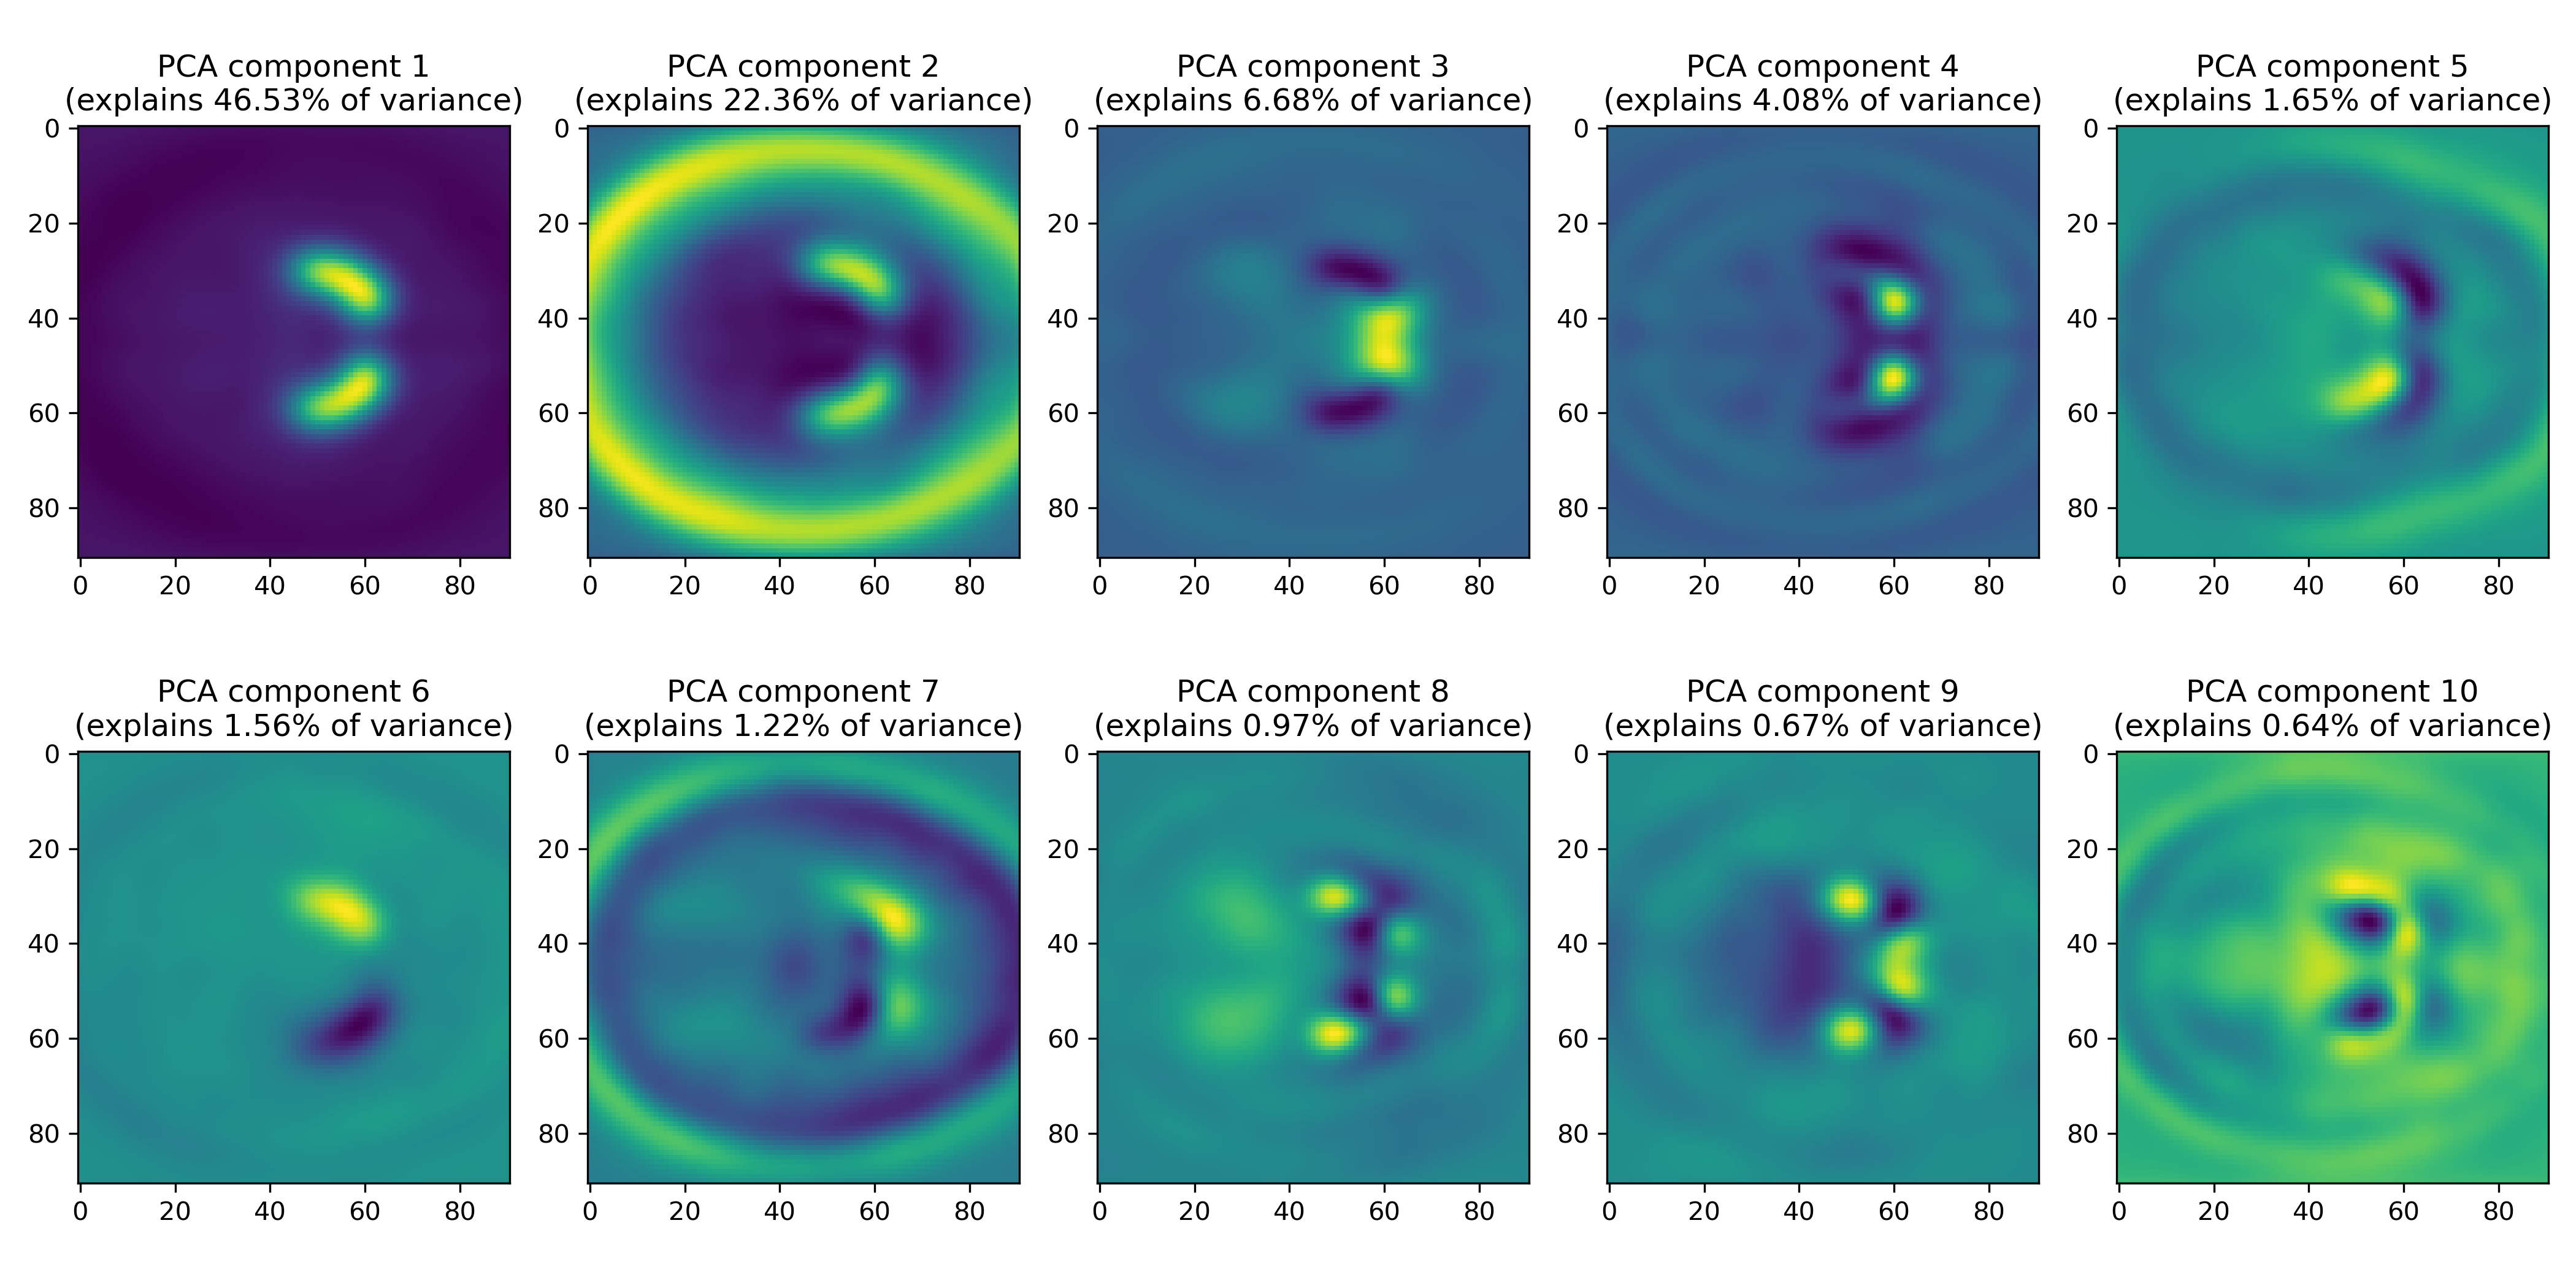
\includegraphics[width=1.0\textwidth]{content/figures/pca_components_splittrain.png}
  \caption{Principle components of the training set (development dataset) for the first random split.} 
  \label{fig:pca_components}
\end{figure} 

\subsection{CNN-based classification}
\label{subsec:cnn_based_classification}

% Model architecture
The models of CNN-based classifiers were based on a Residual Network \\(ResNet) architecture.
More precisely, the \textit{ResNet-18}~\citep{resnet2015} model architecture consisting of 18 layers was used as basis.
The non-pretrained weights of the ResNet-18 were used as initial weights.
The ResNet-18 architecture expects input tensors of size (3, 224, 224), 
denoting images with 3 channels and spatial dimensions of 224 by 224 pixels.
Since the development data has one color channel, the architecture was modified to expect one input channel at its 
first convolutional layer.
Also the dimensions of the last fully-connected layer of the architecture were modified to produce one output node 
in the output layer.
The modified ResNet-18 model is depicted in Figure~\ref{fig:resnet}.
To obtain a probabilistic model output the sigmoid function was applied to the output layer.

% Required preprocessing for CNN: ROI cropping and interpolation to (224, 224)
Further development data preprocessing was performed to comply with the spatial input 
dimensions required by the model architecture.
First, a 91x91 pixel square-shaped region of interest was defined within the 91x109 pixel DVR slab, 
and each development data image (of each subset) was cropped to this region.
The cropping to a square shape was performed to preserve the aspect ratio while doing the subsequent upscaling.
The square-shaped region was determined by cropping an equal number of pixels from the top and bottom 
of the DVR slab along its height dimension.
Then the square-shaped images were resized to the target image size of 224x224 pixels using bicubic interpolation.

The CNN-based approaches were trained for $20$ epochs using a batch size of $64$.
For the MVT and RLT approaches (described in Section~\ref{subsubsec:cnn_based_classification_mvt_rlt}) 
the Binary Cross Entropy (BCE) loss was employed for optimization, 
whereas for the Regression approach (described in Section~\ref{subsubsec:cnn_based_classification_regression}) 
the Mean Squared Error (MSE) loss function was used.
The Adam optimization algorithm was utilized with an initial learning rate of $0.0001$.
During the training of the model, the weights of the best epoch are saved for future evaluation.
Each CNN-based approach was trained and evaluated using identical $10$ random splits of the development data.
Additionally, the trained models were tested on the PPMI and MPH datasets described in Section~\ref{subsec:external_dataset}.

\begin{figure}[t]
  \centering
  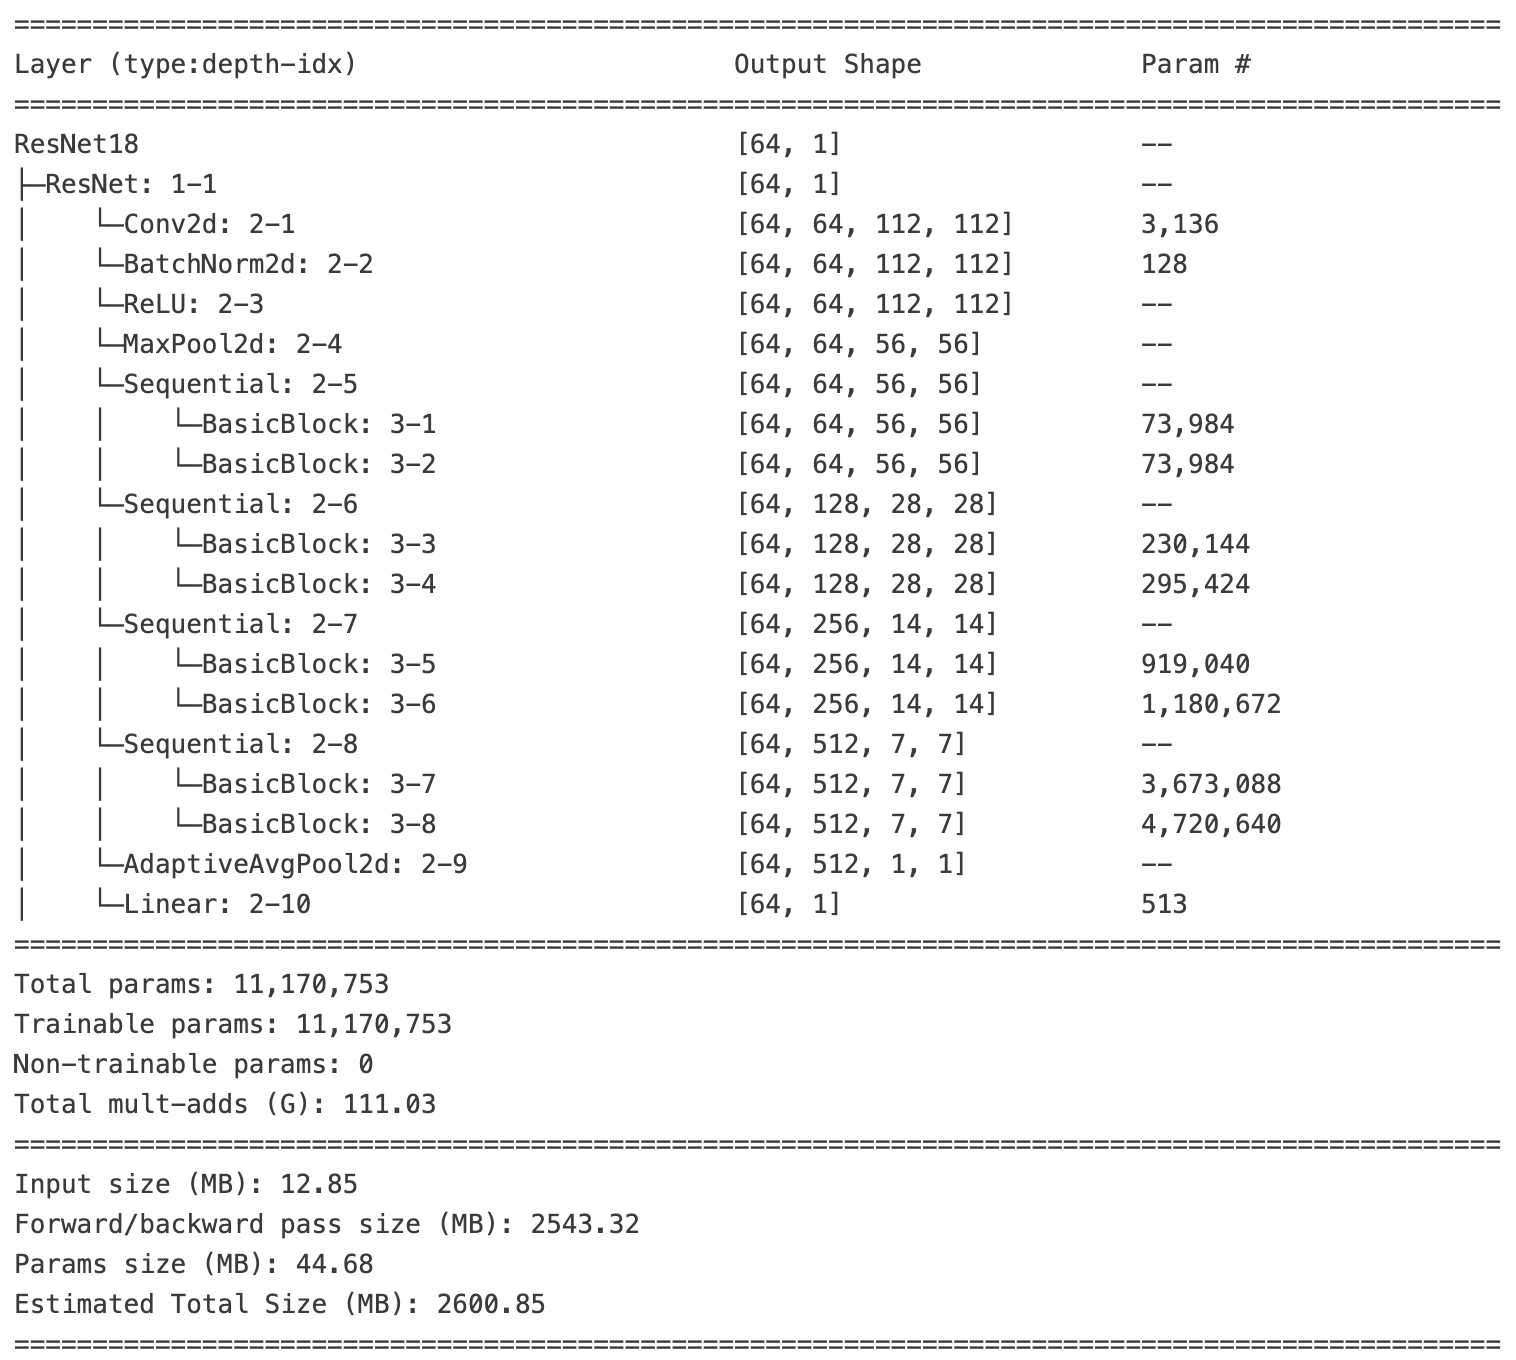
\includegraphics[width=1.0\textwidth]{content/figures/cnn_architecture.png}
  \caption{Overview of the architecture of CNN-based approaches.} 
  \label{fig:resnet}
\end{figure} 

\subsubsection{MVT-based and RLT-based methods}
\label{subsubsec:cnn_based_classification_mvt_rlt}

When training a CNN using the BCE loss function, 
one has to provide the ground truth label of each instance to the optimization algorithm.
Given that each instance in the development data is labeled by three independent readers, 
a selection strategy must be determined.
The following two label selection strategies are used for training the CNNs: 
Majority Vote training (MVT) and “Random Label” training (RLT).
The labels chosen using one of the two strategies are then used, together with the model predictions, 
to compute the BCE loss.

% MVT
Majority vote training involved selecting the label that received the majority of votes from the readers as the 
ground truth label.
Since there are three available labels, 
a majority is reached when two out of the three readers agree on a particular label (e.g., the normal case (NC)).
During the model training phase, the majority vote strategy was employed to select the labels for both the training 
and validation data instances.

% RLT
In contrast to MVT, random label training involved choosing a random label from the three available options
as the ground truth label.
The seed of the random number generator (responsible for the random selection) is set only once at the start of the
algorithm and is not reset between the model training epochs.
Thereby a different label could be chosen as the ground truth label for each distinct training epoch.
Here the random label selection strategy is applied both to the training and validation data.
% majority on validation better?

\subsubsection{Regression-based method}
\label{subsubsec:cnn_based_classification_regression}

The regression-based approach aimed to incorporate the uncertainty regarding the ground truth label 
into the training algorithm.
Therefore, the ground-truth label was derived from the combination of the three available labels, 
resulting in a floating-point number.
Each of the following states of certainty about the label was mapped to a distinct 
floating-point valued ground-truth label: 
\emph{all readers agree on `normal' } (ground-truth label: 0.0), 
\emph{majority of readers (two out of three) agree on `normal'} (ground-truth label: 1.0/3.0), 
\emph{majority of readers (two out of three) agree on `reduced'} (ground-truth label: 2.0/3.0) 
and \emph{all readers agree on `reduced'} (ground-truth label: 1.0).
This mapping of available labels to the ground-truth label was used for both the training 
and validation data during the model training phase.

During model training the loss was computed using the Mean Square Error loss function 
which aims to minimize the mean of the squared differences between the model predictions and the ground-truth labels.
Thereby the optimization algorithm aimed to separate cases where no consensus was reached from those where 
consensus was achieved.

\subsection{Evaluation Metrics and Procedure}
\label{subsec:eval_metrics_proced}

In the following the performance metrics used for the evaluation of the different classification methods 
are explained in more detail.

First the $\text{mean} \pm \text{SD}$ (standard deviation) of the following measures were calculated across
the different random splits for each classification approach and subset (training, validation and testing) given a cutoff: 
Area Under Curve (AUC) for ROC curve, Balanced accuracy, accuracy, sensitivity, specificity, 
Positive Predictive Value (PPV) and Negative Predictive Value (NPV).
The natural cutoff of 0.5 was used for each classification approach except the SBR method.
For the SBR method the optimal cutoff was determined using the Youden criterion~\citep{Youden1950} and was used for
calculating the measures.
Majority vote was used as strategy to assign labels for cases in which no between-reader consensus could be achieved.

% Determination of inconclusive intervals given set of percentages of inconclusive cases
Second for each element within a set of considered percentages of inconclusive cases in the validation set (PIncVal)
the corresponding inconclusive interval was determined.
Inconclusive cases were defined as cases predicted within an inconclusive interval 
(bounded by lower and upper bound), while conclusive cases were those predicted outside this interval.
The determination of the inconclusive interval was exclusively performed using the validation set 
for each random split and classification approach independently.
The set of PIncVal values considered ranged from 0.2\% to 20.0\%, increasing in increments of 0.2\%.
For each target PIncVal value the lower and upper bounds of the inconclusive interval 
were independently determined in such a way that there was a similar number of inconclusive cases both below and above 
the pre-defined cutoff.
For the CNN-based classification approaches (described in Section~\ref{subsec:cnn_based_classification}) and the 
multivariate benchmark (described in Section~\ref{subsec:pca_rfc}) the natural cutoff of 0.5 was used.
For the SBR-based univariate benchmark (described in Section~\ref{subsec:sbr}), 
the optimal cutoff on the SBR obtained by applying the Youden criterion~\citep{Youden1950} using ROC analysis was used.

% lower_bound(PIncVal) , upper_bound(PIncVal)
To assess the stability of the determined inconclusive interval over the proportion of inconclusive cases
the determined upper and lower bounds ($\text{mean} \pm \text{SD}$) of the inconclusive interval
were plotted against the corresponding PIncVal (\%).
The $\text{mean} \pm \text{SD}$ of determined upper and lower bounds was calculated across the measures for 
different random splits.
The rate at which the lower (upper) bound decreases (increases) over the PIncVal 
reflects the density of inconclusive cases within a certain region of PIncVal.
Specifically, higher function gradients indicate lower concentration of predictions, 
and vice versa.
Also a higher standard deviation from the mean indicates that a stable inconclusive interval determination 
is harder within a certain region of PIncVal.
The measurement was conducted separately for each classification approach.

% AUC of bal_acc vs. %inconclusive_cases; determination of inconclusive ranges for each %inconclusive_cases

As the main performance metric used in this work to evaluate and compare the classification approaches 
we propose the area under the curve (AUC) of mean balanced accuracy (\%) on conclusive test cases as a function of 
the mean percentage of inconclusive test cases (mean PIncObs, \%).
More precisely the relative AUC (\%) normalized to the maximum achievable area was used for the comparison.
To obtain the relative AUC, 
first, the mean balanced accuracy function was interpolated using cubic spline interpolation.
Then the area under the mean balanced accuracy curve was computed using the trapezoidal rule 
and then normalized to the maximum achievable area.
The evaluation of each classification method with respect to this metric was conducted on the test set of the 
development dataset as well as on the independent datasets PPMI and MPH.

% PIncObs(PIncVal) 
As a further metric, the $\text{mean} \pm \text{SD}$ percentage of observed inconclusive cases in the test set (PIncObs, \%) 
was plotted against the PIncVal (\%).
A mean of PIncObs(PIncVal) near the identity line is an indicator for a similar prediction distribution 
for validation set and test set on average.
In case the mean of PIncObs(PIncVal) consistently lies over (under) the identity line 
the supposed prediction certainty on the test set, on average, is lower (higher) than on the validation set.
Also a lower standard deviation of PIncObs over PIncVal indicates 
that PIncObs is less sensitive to the randomness of the inconclusive intervals across random splits.
Therefore a lower standard deviation of PIncObs allows for a more reliable main performance metric calculation.


\section{Data Sources}
\label{sec:data}

The study retrospectively included 3 different datasets with a total of 3025 DAT-SPECT images.
The primary dataset (`development dataset') was used for both training and testing the models associated with the respective method, 
whereas the other two datasets, the \textit{PPMI} dataset and the \textit{MPH} dataset were used for testing only, not for training.

\subsection{Development dataset}
\label{subsec:spect_dataset}

The development dataset consisted of 1740 consecutive DAT-SPECT scans obtained from clinical routine at 
the Department of Nuclear Medicine, University Medical Center Hamburg-Eppendorf~\citep{Schiebler2023}.
In brief, DAT-SPECT with [$^{123}$I]FP-CIT had been performed according to common procedures guidelines~\citep{Darcourt2010-ar, Djang2012-ow} 
with different double-head cameras equipped with low-energy-high-resolution or fan-beam collimators. 
The projection data were reconstructed using the iterative ordered-subsets-expectation-maximization~\citep{Hudson1994} 
with attenuation and simulation-based scatter correction 
as well as collimator-detector response modeling as implemented in the Hybrid Recon-Neurology tool 
of the Hermes SMART workstation v1.6 (Hermes Medical Solutions, Stockholm, Sweden)~\citep{Diemling2021-mg, Sohlberg2012-ep, HybridRecon, Kangasmaa2016-aw}.
All parameter settings were as recommended by Hermes~\citep{Diemling2021-mg} for the EANM / EANM Research Ltd (EARL) ENC-DAT project (European Normal Control Database of DaTSCAN)~\citep{Tossici-Bolt2011-cx, Dickson2010-fm, Varrone2013-it, Tossici-Bolt2017-xj, Dickson2012-hk}.
More precisely, ordered-subsets-expectation-maximization was performed with 5 iterations and 15/16 subsets for 120/128 views. 
For noise suppression, reconstructed images were postfiltered by convolution with a 3-dimensional Gaussian kernel of 7 mm full-width-at-half-maximum. 

The ground-truth label, indicating either `normal' or `Parkinson-typical' reduction (`reduced') of the striatal signal, 
was obtained by visual assessment of the DAT-SPECT images by three independent readers~\citep{Schiebler2023}. 
The readers achieved inter-reader consensus on the `normal' label in 855 cases ($49.1\%$)
and on the `reduced' label in 802 cases ($46.1\%$).
The inter-reader consensus on the label could not be achieved for 83 cases ($4.8\%$).
The dataset comprised about $43.5\%$ female cases and $56.5\%$ male cases.
In the dataset, the average age among cases was $66.7$ with a standard deviation of $11.6$ years.
The development dataset was utilized for both training and testing the classification models. 

\subsection{Independent testing datasets}
\label{subsec:external_dataset}

The second dataset comprised 645 DAT-SPECT with [$^{123}$I]FP-CIT from the Parkinson's Progression Markers Initiative (PPMI) 
(www.ppmi-info.org/data)~\citep{Parkinson_Progression_Marker_Initiative2011-px}.
The external dataset included 438 patients with Parkinson's disease and 207 healthy controls as described in~\cite{Wenzel2019}.
The mean age among cases was $61.2$ with a standard deviation of $10.2$ years, 
and the dataset comprised $35.2\%$ female cases.
Details of the PPMI DAT-SPECT protocol are given at http://www.ppmi-info.org/study-design/research-documents-and-sops/ ~\citep{Parkinson_Progression_Marker_Initiative2011-px}. 
Raw projection data has been transferred to the PPMI imaging core lab for central image reconstruction using an iterative (HOSEM) algorithm on a HERMES workstation. 
The clinical diagnosis was used as ground-truth label (Parkinson's disease = ``reduced", healthy control = ``normal"). 
The external dataset showed lower spatial resolution than the development dataset (lower striatum-to-background contrast).

The third dataset (`MPH dataset') comprised 640 consecutive DAT-SPECT with [$^{123}$I]FP-CIT from clinical routine at UKE 
that had been acquired with a triple-head camera equipped with brain-specific multiple pinhole (MPH) collimators. 
Multiple pinhole SPECT concurrently improves count sensitivity and spatial resolution compared to SPECT with parallel-hole 
and fan-beam collimators~\citep{Mathies2022-yi, Tecklenburg2020-xr}.
The projection data were reconstructed with the Monte Carlo photon simulation engine 
and iterative one-step-late maximum-a-posteriori expectation-maximization implemented 
in the camera software (24 iterations, 2 subsets)~\citep{Tecklenburg2020-xr, Magdics2010}.
Neither attenuation nor scatter correction was applied to the SPECT images.
The ground-truth label (`normal' or `reduced') was obtained by the visual interpretation of an experienced reader 
(about 20 years of experience in clinical DAT-SPECT reading, $\geq$3,000 cases).
All SPECT images were interpreted twice (with different randomization) by the same reader. 
The delay between the reading sessions was 14 days. 
Cases with discrepant interpretations between the two reading sessions were read a third time by the same reader 
to obtain an intra-reader consensus as the ground-truth label. 
Thereby 327 cases ($51.1\%$) were labeled as `reduced'  and 313 cases ($48.9\%$) were labeled as `normal'.
The dataset contained 283 female cases ($44.2\%$),
and the average age among cases was $67.2$ with a standard deviation of $11.4$ years.
In contrast to the development dataset, the internal test dataset exhibited a better spatial resolution, 
leading to higher contrast between the striatum and background, along with reduced statistical noise.
The MPH dataset has not been described in previous works.

Figure~\ref{fig:datasets_samples} illustrates example DVR slabs for one `normal' case and three `reduced' cases obtained
from the development dataset, the PPMI dataset, and the MPH dataset.

\begin{figure}[t]
    \centering
    \colorbox{black}{%
     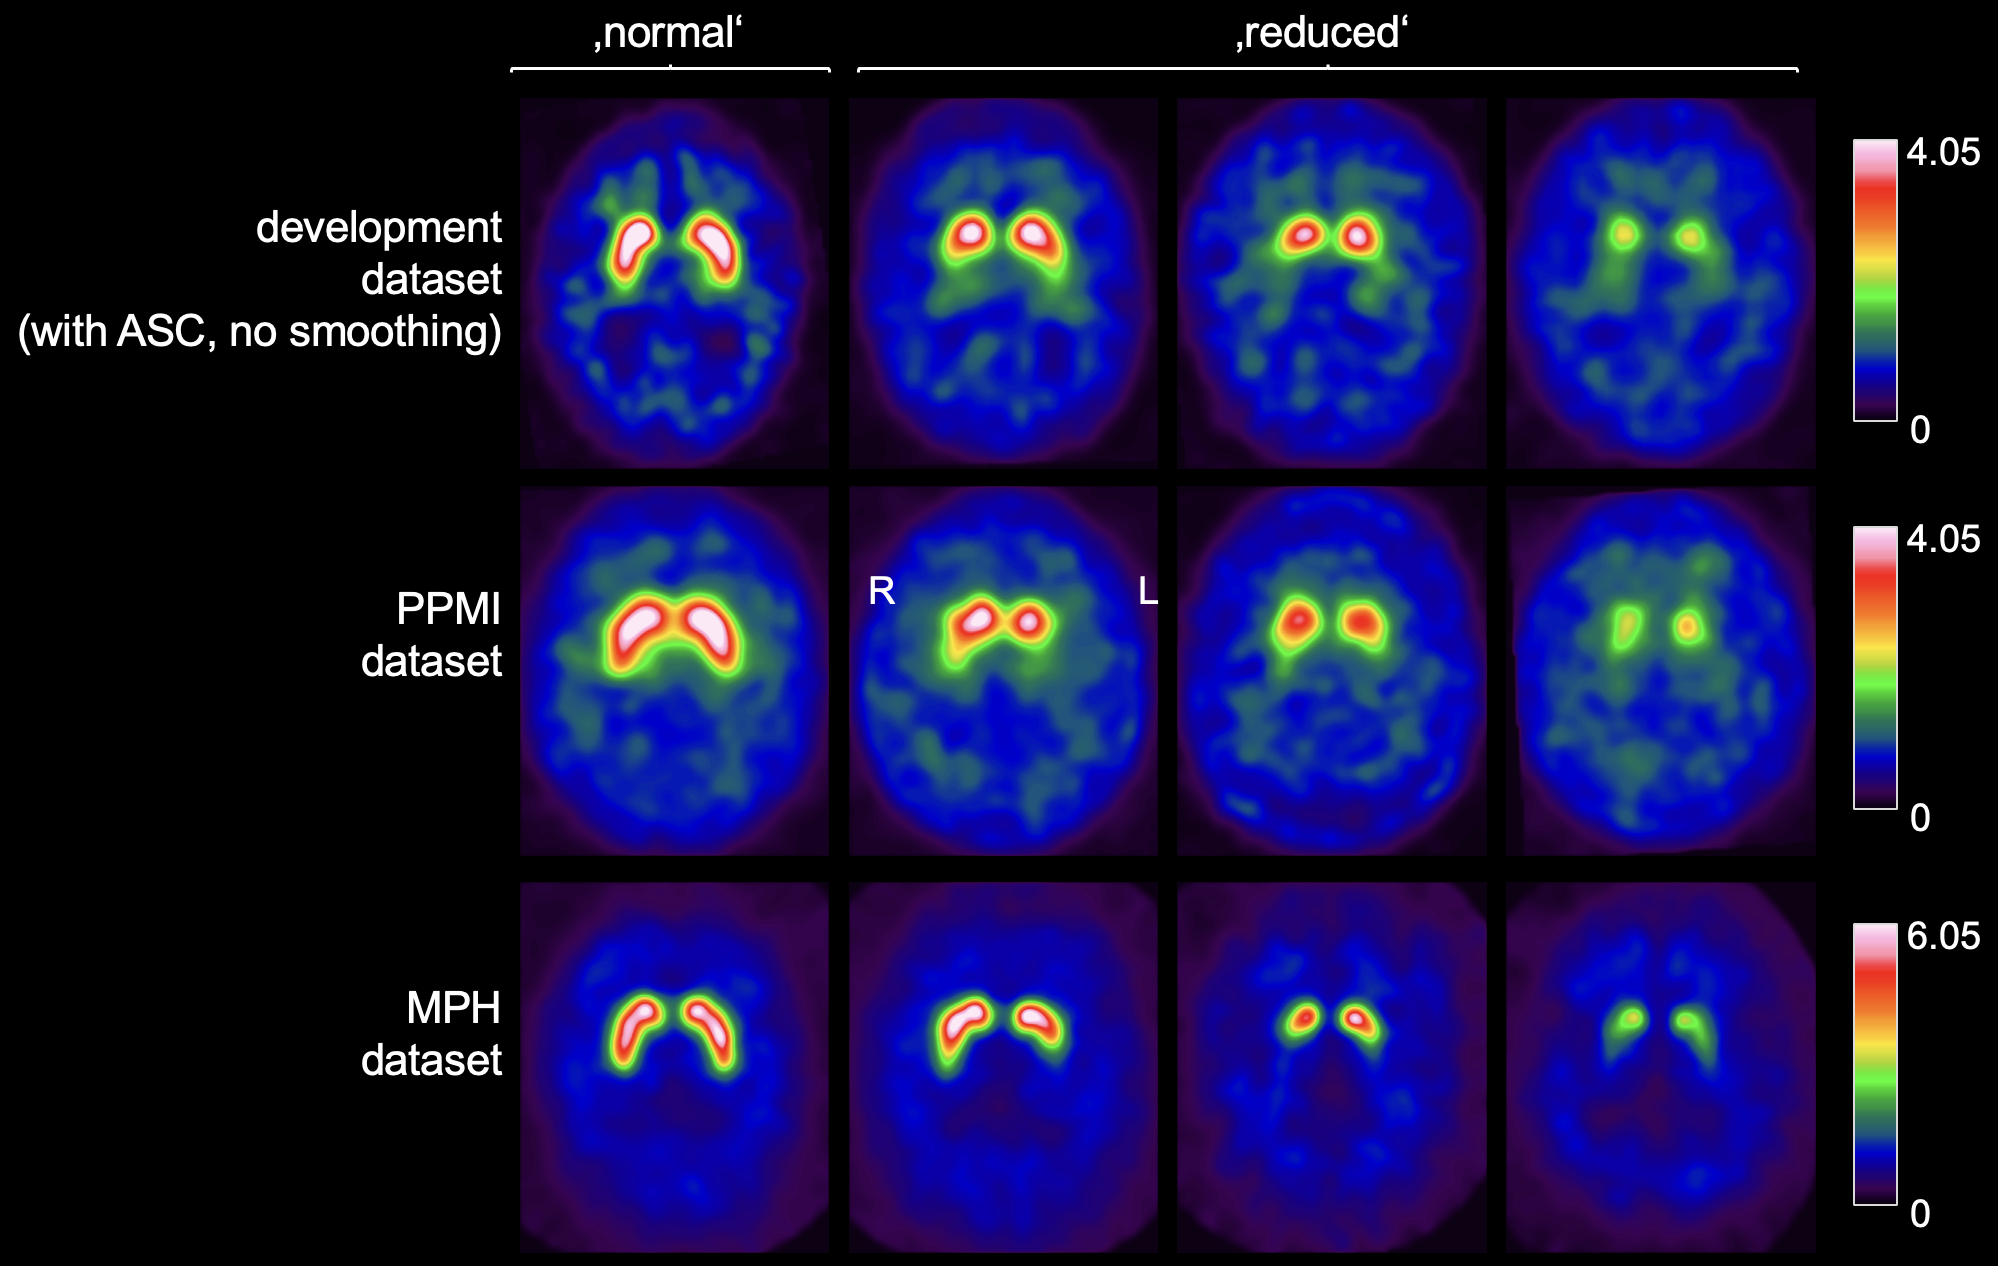
\includegraphics[width=0.95\textwidth]{content/figures/datasets_samples.png}%
     }
    \caption{DVR slabs for one healthy control (`normal') case 
    and three cases with reduced availability of DAT in the striatum (`reduced')
    from the development dataset, the PPMI dataset, and the MPH dataset.
    For the cases from the development dataset, attenuation and scatter correction (ASC) were applied, 
    and no smoothing was performed.} 
    \label{fig:datasets_samples}
\end{figure}


\section{Evaluation}
\label{sec:evaluation}

The preceding chapters have detailed the research methodology, data collection and sources, and the application of classification techniques 
to address the research questions posed in this study. 

This chapter embarks on the evaluation of the research results, focusing on the performance and effectiveness of the methods employed, 
and the attainment of the research objectives.

The structure of this chapter has been designed to systematically lead readers through the assessment process. 
It commences with a discussion of the research objectives that serve as the focal points for subsequent evaluations. 
Following this, a comprehensive examination of performance metrics is conducted, with an emphasis on their 
significance within the context of this research, providing detailed insights into the criteria employed 
to evaluate research outcomes.
The core of this chapter subsequently unveils the experimental results encompassing various test datasets 
and classification methods. 
These findings are presented using graphical representations and supported by a range of statistical measures.
The chapter culminates with a comparative analysis, which seeks to assess and contrast the effectiveness and 
limitations of the research methods employed.

\subsection{Research Objectives}
\label{subsec:research_objectives}

% TODO

% Objective 1: Evaluation of Methods on Test set of dev data

%   Objective 1.1: To compare the "performance" of the methods on Test set of dev data.
%   Objective 1.2: To assess the suitability of these methods in unseen real-world scenarios


% Objective 2: Evaluation of Methods on PPMI and MPH dataset
%				-> understand the impact of varying dataset characteristics by evaluating on


\subsection{Evaluation Metrics and Procedure}
\label{subsec:determinationInconcl}

In the following the performance metrics used for the evaluation of the different classification methods 
are explained in more detail.

First the $\text{mean} \pm \text{SD}$ (standard deviation) of the following measures were calculated across
the different random splits for each classification approach given a cutoff: 
Area Under Curve (AUC) for ROC curve, Balanced accuracy, accuracy, sensitivity, specificity, 
Positive Predictive Value (PPV) and Negative Predictive Value (NPV).
The natural cutoff of 0.5 was used for each classification approach except the SBR method.
For the SBR method the optimal cutoff was determined using the Youden criterion~\citep{Youden1950} and was used for
calculating the measures.

% Determination of inconclusive intervals given set of percentages of inconclusive cases
Second for each element within a set of considered percentages of inconclusive cases in the validation set 
the corresponding inconclusive interval was determined.
Inconclusive cases were defined as cases predicted within an inconclusive interval 
(bounded by lower and upper bound), while conclusive cases were those predicted outside this interval.
The determination of the inconclusive interval was exclusively performed using the validation set 
for each random split and classification approach independently.
The set of percentages of inconclusive cases considered ranged from 0.2\% to 20.0\%, increasing in increments of 0.2\%.
For each target percentage of inconclusive cases in the set the lower and upper bounds of the inconclusive interval 
were independently determined in such a way that there was a similar number of inconclusive cases both below and above 
the pre-defined cutoff.
For the CNN-based classification approaches (described in Section~\ref{subsec:cnn_based_classification}) and the 
multivariate benchmark (described in Section~\ref{subsec:pca_rfc}) the natural cutoff of 0.5 was used.
For the SBR-based univariate benchmark (described in Section~\ref{subsec:sbr}), 
the optimal cutoff on the SBR obtained by applying the Youden criterion~\citep{Youden1950} using ROC analysis was used.

% Stability of inconclusive interval
To assess the stability of the determined inconclusive interval over the proportion of inconclusive cases
the determined upper and lower bounds ($\text{mean} \pm \text{SD}$) of the inconclusive interval
were plotted against the corresponding proportion of inconclusive cases (\%) in the validation set.
The $\text{mean} \pm \text{SD}$ of determined upper and lower bounds was calculated across the measures for 
different random splits.
The rate at which the lower (upper) bound decreases (increases) in relation to the proportion of inconclusive 
cases reflects the density of inconclusive cases around the cutoff.
Specifically, higher function gradients indicate lower concentration of predictions around the cutoff, 
and vice versa.
The measurement was conducted separately for each classification approach.

% AUC of bal_acc vs. %inconclusive_cases; determination of inconclusive ranges for each %inconclusive_cases

The main performance metric used in this work to evaluate and compare the classification approaches was 
the area under the curve (AUC) of mean balanced accuracy (\%) on conclusive test cases as a function of 
the proportion of inconclusive test cases (\%, mean).
More precisely the relative AUC (\%) normalized to the maximum achievable area was used for the comparison.
To obtain the relative AUC, 
first, the mean balanced accuracy function was interpolated using cubic spline interpolation.
Then the area under the mean balanced accuracy curve was computed using the trapezoidal rule 
and then normalized to the maximum achievable area.
The evaluation of each classification method with respect to this metric was conducted on the test set of the 
development dataset as well as on the independent datasets PPMI and MPH."


% Proportion of inconclusive cases in test set vs. 
Also the observed $\text{mean} \pm \text{SD}$ proportion of inconclusive cases in the test set was plotted 
against the proportion of inconclusive cases in the validation set.
% WHY? Explain what would indicate desired behaviour and what not


%%%%%%%%%%%%%%%%%%%%%%%%%%%%%%%%%%%%%%%%%%%%%%%%%%%%%%%%%%%%%%%%%%%%%%%%%%%%%%%%%%%%%%%%%%%%%%%%%%%%%%%%%%%%%%%%%%%%%%%

\subsection{Evaluation of SBR Method}
\label{subsec:eval_sbr}

%%%%%%%%%%%%%%%%%%%%%%%%%%%%%%%%%%%%%%%%%%%%%%%%%%%%%%%%%%%%%%%%%%%%%%%%%%%%%%%%%%%%%%%%%%%%%%%%%%%%%%%%%%%%%%%%%%%%%%%

% Evaluation on Development dataset

% sbr_percInconclCases_development
\begin{figure}[t]
    \centering
    \includegraphics[width=1.0\textwidth]{content/figures/evaluations/sbr/86/sbr_percInconclCases_development.png}
    \caption{Evaluation of the SBR method on Test Set of Development Dataset. 
    Determined upper and lower bounds of the inconclusive interval as a function of the percentage of inconclusive cases.} 
    \label{fig:sbr_percInconclCases_development}
\end{figure}


% obsInconclCases_inconclCasesValid_sbr_development
\begin{figure}[h]
    \centering
    \includegraphics[width=1.0\textwidth]{content/figures/evaluations/sbr/86/obsInconclCases_inconclCasesValid_sbr_development.png}
    \caption{Evaluation of the SBR method on Test Set of Development Dataset.
    Observed percentage of inconclusive cases in the test set 
    for a given set of percentages of inconclusive cases in the validation set.
    Each of the percentages of inconclusive cases in the validation set is associated 
    with an inconclusive range (determined in the validation set).} 
    \label{fig:obsInconclCases_inconclCasesValid_sbr_development}
\end{figure} 


% bacc_obsInconclCases_sbr_development_full
\begin{figure}[t]
    \begin{subfigure}{0.9\textwidth}
      \centering
      \includegraphics[width=0.9\textwidth]{content/figures/evaluations/sbr/86/bacc_obsInconclCases_sbr_development.png}
      \subcaption{}
      \label{fig:bacc_obsInconclCases_sbr_development}
    \end{subfigure}
    \hfill
    \begin{subfigure}{0.9\textwidth}
      \centering
      \includegraphics[width=0.9\textwidth]{content/figures/evaluations/sbr/86/bacc_obsInconclCases_concl_sbr_development.png}
      \subcaption{}
      \label{fig:bacc_obsInconclCases_concl_sbr_development}
    \end{subfigure}

    \caption{Evaluation of the SBR method on Test Set of Development Dataset.
    Balanced accuracy for a given mean percentage of observed inconclusive cases in the test set on 
    (a) both conclusive and inconclusive cases and (b) only conclusive cases. 
    Each of the mean percentages of observed inconclusive cases is associated with an inconclusive range (determined in the validation set). }
    \label{fig:bacc_obsInconclCases_sbr_development_full}
\end{figure}

%%%%%%%%%%%%%%%%%%%%%%%%%%%%%%%%%%%%%%%%%%%%%%%%%%%%%%%%%%%%%%%%%%%%%%%%%%%%%%%%%%%%%%%%%%%%%%%%%%%%%%%%%%%%%%%%%%%%%%%

% Evaluation on Independent datasets

% ---------------- PPMI ---------------------

% obsInconclCases_inconclCasesValid_sbr_ppmi
\begin{figure}[h]
  \centering
  \includegraphics[width=1.0\textwidth]{content/figures/evaluations/sbr/86/obsInconclCases_inconclCasesValid_sbr_ppmi.png}
  \caption{Evaluation of the SBR method on PPMI Dataset.
  Observed percentage of inconclusive cases in the PPMI dataset 
  for a given set of percentages of inconclusive cases in the validation set (Development Dataset).
  Each of the percentages of inconclusive cases in the validation set is associated 
  with an inconclusive range (determined in the validation set).} 
  \label{fig:obsInconclCases_inconclCasesValid_sbr_ppmi}
\end{figure} 


% bacc_obsInconclCases_sbr_ppmi_full
\begin{figure}[t]
  \begin{subfigure}{0.9\textwidth}
    \centering
    \includegraphics[width=0.9\textwidth]{content/figures/evaluations/sbr/86/bacc_obsInconclCases_sbr_ppmi.png}
    \subcaption{}
    \label{fig:bacc_obsInconclCases_sbr_ppmi}
  \end{subfigure}
  \hfill
  \begin{subfigure}{0.9\textwidth}
    \centering
    \includegraphics[width=0.9\textwidth]{content/figures/evaluations/sbr/86/bacc_obsInconclCases_concl_sbr_ppmi.png}
    \subcaption{}
    \label{fig:bacc_obsInconclCases_concl_sbr_ppmi}
  \end{subfigure}

  \caption{Evaluation of the SBR method on PPMI Dataset.
  Balanced accuracy for a given mean percentage of inconclusive cases observed in the PPMI dataset on 
  (a) both conclusive and inconclusive cases and (b) only conclusive cases. 
  Each of the mean percentages of observed inconclusive cases is associated 
  with an inconclusive range (determined in the validation set). }
  \label{fig:bacc_obsInconclCases_sbr_ppmi_full}
\end{figure}



% -------------- MPH -----------------


% obsInconclCases_inconclCasesValid_sbr_mph
\begin{figure}[h]
  \centering
  \includegraphics[width=1.0\textwidth]{content/figures/evaluations/sbr/86/obsInconclCases_inconclCasesValid_sbr_mph.png}
  \caption{Evaluation of the SBR method on MPH Dataset.
  Observed percentage of inconclusive cases in the MPH dataset 
  for a given set of percentages of inconclusive cases in the validation set (Development Dataset).
  Each of the percentages of inconclusive cases in the validation set is associated 
  with an inconclusive range (determined in the validation set).} 
  \label{fig:obsInconclCases_inconclCasesValid_sbr_mph}
\end{figure} 


% bacc_obsInconclCases_sbr_mph_full
\begin{figure}[t]
  \begin{subfigure}{0.9\textwidth}
    \centering
    \includegraphics[width=0.9\textwidth]{content/figures/evaluations/sbr/86/bacc_obsInconclCases_sbr_mph.png}
    \subcaption{}
    \label{fig:bacc_obsInconclCases_sbr_mph}
  \end{subfigure}
  \hfill
  \begin{subfigure}{0.9\textwidth}
    \centering
    \includegraphics[width=0.9\textwidth]{content/figures/evaluations/sbr/86/bacc_obsInconclCases_concl_sbr_mph.png}
    \subcaption{}
    \label{fig:bacc_obsInconclCases_concl_sbr_mph}
  \end{subfigure}

  \caption{Evaluation of the SBR method on MPH Dataset.
  Balanced accuracy for a given mean percentage of inconclusive cases observed in the MPH dataset on 
  (a) both conclusive and inconclusive cases and (b) only conclusive cases. 
  Each of the mean percentages of observed inconclusive cases is associated 
  with an inconclusive range (determined in the validation set). }
  \label{fig:bacc_obsInconclCases_sbr_mph_full}
\end{figure}



%%%%%%%%%%%%%%%%%%%%%%%%%%%%%%%%%%%%%%%%%%%%%%%%%%%%%%%%%%%%%%%%%%%%%%%%%%%%%%%%%%%%%%%%%%%%%%%%%%%%%%%%%%%%%%%%%%%%%%%

\subsection{Evaluation of Random Forest Method}
\label{subsec:eval_rfc}


%%%%%%%%%%%%%%%%%%%%%%%%%%%%%%%%%%%%%%%%%%%%%%%%%%%%%%%%%%%%%%%%%%%%%%%%%%%%%%%%%%%%%%%%%%%%%%%%%%%%%%%%%%%%%%%%%%%%%%%

% Evaluation on Development dataset

% pca_rfc_percInconclCases_development
\begin{figure}[t]
  \centering
  \includegraphics[width=1.0\textwidth]{content/figures/evaluations/pca_rfc/86/sigmoid_percInconclCases_pca_rfc_development.png}
  \caption{Evaluation of the PCA-RFC method on Test Set of Development Dataset. 
  Determined upper and lower bounds of the inconclusive interval as a function of the percentage of inconclusive cases.} 
  \label{fig:pca_rfc_percInconclCases_development}
\end{figure}


% obsInconclCases_inconclCasesValid_pca_rfc_development
\begin{figure}[h]
  \centering
  \includegraphics[width=1.0\textwidth]{content/figures/evaluations/pca_rfc/86/obsInconclCases_inconclCasesValid_pca_rfc_development.png}
  \caption{Evaluation of the PCA-RFC method on Test Set of Development Dataset.
  Observed percentage of inconclusive cases in the test set 
  for a given set of percentages of inconclusive cases in the validation set.
  Each of the percentages of inconclusive cases in the validation set is associated 
  with an inconclusive range (determined in the validation set).} 
  \label{fig:obsInconclCases_inconclCasesValid_pca_rfc_development}
\end{figure} 


% bacc_obsInconclCases_pca_rfc_development_full
\begin{figure}[t]
  \begin{subfigure}{0.9\textwidth}
    \centering
    \includegraphics[width=0.9\textwidth]{content/figures/evaluations/pca_rfc/86/bacc_obsInconclCases_pca_rfc_development.png}
    \subcaption{}
    \label{fig:bacc_obsInconclCases_pca_rfc_development}
  \end{subfigure}
  \hfill
  \begin{subfigure}{0.9\textwidth}
    \centering
    \includegraphics[width=0.9\textwidth]{content/figures/evaluations/pca_rfc/86/bacc_obsInconclCases_concl_pca_rfc_development.png}
    \subcaption{}
    \label{fig:bacc_obsInconclCases_concl_pca_rfc_development}
  \end{subfigure}

  \caption{Evaluation of the PCA-RFC method on Test Set of Development Dataset.
  Balanced accuracy for a given mean percentage of observed inconclusive cases in the test set on 
  (a) both conclusive and inconclusive cases and (b) only conclusive cases. 
  Each of the mean percentages of observed inconclusive cases is associated with an inconclusive range (determined in the validation set). }
  \label{fig:bacc_obsInconclCases_pca_rfc_development_full}
\end{figure}

%%%%%%%%%%%%%%%%%%%%%%%%%%%%%%%%%%%%%%%%%%%%%%%%%%%%%%%%%%%%%%%%%%%%%%%%%%%%%%%%%%%%%%%%%%%%%%%%%%%%%%%%%%%%%%%%%%%%%%%

% Evaluation on Independent datasets

% ---------------- PPMI ---------------------

% obsInconclCases_inconclCasesValid_pca_rfc_ppmi
\begin{figure}[h]
\centering
\includegraphics[width=1.0\textwidth]{content/figures/evaluations/pca_rfc/86/obsInconclCases_inconclCasesValid_pca_rfc_ppmi.png}
\caption{Evaluation of the PCA-RFC method on PPMI Dataset.
Observed percentage of inconclusive cases in the PPMI dataset 
for a given set of percentages of inconclusive cases in the validation set (Development Dataset).
Each of the percentages of inconclusive cases in the validation set is associated 
with an inconclusive range (determined in the validation set).} 
\label{fig:obsInconclCases_inconclCasesValid_pca_rfc_ppmi}
\end{figure} 


% bacc_obsInconclCases_pca_rfc_ppmi_full
\begin{figure}[t]
\begin{subfigure}{0.9\textwidth}
  \centering
  \includegraphics[width=0.9\textwidth]{content/figures/evaluations/pca_rfc/86/bacc_obsInconclCases_pca_rfc_ppmi.png}
  \subcaption{}
  \label{fig:bacc_obsInconclCases_pca_rfc_ppmi}
\end{subfigure}
\hfill
\begin{subfigure}{0.9\textwidth}
  \centering
  \includegraphics[width=0.9\textwidth]{content/figures/evaluations/pca_rfc/86/bacc_obsInconclCases_concl_pca_rfc_ppmi.png}
  \subcaption{}
  \label{fig:bacc_obsInconclCases_concl_pca_rfc_ppmi}
\end{subfigure}

\caption{Evaluation of the PCA-RFC method on PPMI Dataset.
Balanced accuracy for a given mean percentage of inconclusive cases observed in the PPMI dataset on 
(a) both conclusive and inconclusive cases and (b) only conclusive cases. 
Each of the mean percentages of observed inconclusive cases is associated 
with an inconclusive range (determined in the validation set). }
\label{fig:bacc_obsInconclCases_pca_rfc_ppmi_full}
\end{figure}



% -------------- MPH -----------------


% obsInconclCases_inconclCasesValid_pca_rfc_mph
\begin{figure}[h]
\centering
\includegraphics[width=1.0\textwidth]{content/figures/evaluations/pca_rfc/86/obsInconclCases_inconclCasesValid_pca_rfc_mph.png}
\caption{Evaluation of the PCA-RFC method on MPH Dataset.
Observed percentage of inconclusive cases in the MPH dataset 
for a given set of percentages of inconclusive cases in the validation set (Development Dataset).
Each of the percentages of inconclusive cases in the validation set is associated 
with an inconclusive range (determined in the validation set).} 
\label{fig:obsInconclCases_inconclCasesValid_pca_rfc_mph}
\end{figure} 


% bacc_obsInconclCases_pca_rfc_mph_full
\begin{figure}[t]
\begin{subfigure}{0.9\textwidth}
  \centering
  \includegraphics[width=0.9\textwidth]{content/figures/evaluations/pca_rfc/86/bacc_obsInconclCases_pca_rfc_mph.png}
  \subcaption{}
  \label{fig:bacc_obsInconclCases_pca_rfc_mph}
\end{subfigure}
\hfill
\begin{subfigure}{0.9\textwidth}
  \centering
  \includegraphics[width=0.9\textwidth]{content/figures/evaluations/pca_rfc/86/bacc_obsInconclCases_concl_pca_rfc_mph.png}
  \subcaption{}
  \label{fig:bacc_obsInconclCases_concl_pca_rfc_mph}
\end{subfigure}

\caption{Evaluation of the PCA-RFC method on MPH Dataset.
Balanced accuracy for a given mean percentage of inconclusive cases observed in the MPH dataset on 
(a) both conclusive and inconclusive cases and (b) only conclusive cases. 
Each of the mean percentages of observed inconclusive cases is associated 
with an inconclusive range (determined in the validation set). }
\label{fig:bacc_obsInconclCases_pca_rfc_mph_full}
\end{figure}



\subsection{Evaluation of MVT-based Method}
\label{subsec:eval_mvt}



%%%%%%%%%%%%%%%%%%%%%%%%%%%%%%%%%%%%%%%%%%%%%%%%%%%%%%%%%%%%%%%%%%%%%%%%%%%%%%%%%%%%%%%%%%%%%%%%%%%%%%%%%%%%%%%%%%%%%%%

% Evaluation on Development dataset

% baseline_majority_percInconclCases_development
\begin{figure}[t]
  \centering
  \includegraphics[width=1.0\textwidth]{content/figures/evaluations/baseline_majority/86/sigmoid_percInconclCases_baseline_majority_development.png}
  \caption{Evaluation of the CNN-MVT method on Test Set of Development Dataset. 
  Determined upper and lower bounds of the inconclusive interval as a function of the percentage of inconclusive cases.} 
  \label{fig:baseline_majority_percInconclCases_development}
\end{figure}


% obsInconclCases_inconclCasesValid_baseline_majority_development
\begin{figure}[h]
  \centering
  \includegraphics[width=1.0\textwidth]{content/figures/evaluations/baseline_majority/86/obsInconclCases_inconclCasesValid_baseline_majority_development.png}
  \caption{Evaluation of the CNN-MVT method on Test Set of Development Dataset.
  Observed percentage of inconclusive cases in the test set 
  for a given set of percentages of inconclusive cases in the validation set.
  Each of the percentages of inconclusive cases in the validation set is associated 
  with an inconclusive range (determined in the validation set).} 
  \label{fig:obsInconclCases_inconclCasesValid_baseline_majority_development}
\end{figure} 


% bacc_obsInconclCases_baseline_majority_development_full
\begin{figure}[t]
  \begin{subfigure}{0.9\textwidth}
    \centering
    \includegraphics[width=0.9\textwidth]{content/figures/evaluations/baseline_majority/86/bacc_obsInconclCases_baseline_majority_development.png}
    \subcaption{}
    \label{fig:bacc_obsInconclCases_baseline_majority_development}
  \end{subfigure}
  \hfill
  \begin{subfigure}{0.9\textwidth}
    \centering
    \includegraphics[width=0.9\textwidth]{content/figures/evaluations/baseline_majority/86/bacc_obsInconclCases_concl_baseline_majority_development.png}
    \subcaption{}
    \label{fig:bacc_obsInconclCases_concl_baseline_majority_development}
  \end{subfigure}

  \caption{Evaluation of the CNN-MVT method on Test Set of Development Dataset.
  Balanced accuracy for a given mean percentage of observed inconclusive cases in the test set on 
  (a) both conclusive and inconclusive cases and (b) only conclusive cases. 
  Each of the mean percentages of observed inconclusive cases is associated with an inconclusive range (determined in the validation set). }
  \label{fig:bacc_obsInconclCases_baseline_majority_development_full}
\end{figure}

%%%%%%%%%%%%%%%%%%%%%%%%%%%%%%%%%%%%%%%%%%%%%%%%%%%%%%%%%%%%%%%%%%%%%%%%%%%%%%%%%%%%%%%%%%%%%%%%%%%%%%%%%%%%%%%%%%%%%%%

% Evaluation on Independent datasets

% ---------------- PPMI ---------------------

% obsInconclCases_inconclCasesValid_baseline_majority_ppmi
\begin{figure}[h]
\centering
\includegraphics[width=1.0\textwidth]{content/figures/evaluations/baseline_majority/86/obsInconclCases_inconclCasesValid_baseline_majority_ppmi.png}
\caption{Evaluation of the CNN-MVT method on PPMI Dataset.
Observed percentage of inconclusive cases in the PPMI dataset 
for a given set of percentages of inconclusive cases in the validation set (Development Dataset).
Each of the percentages of inconclusive cases in the validation set is associated 
with an inconclusive range (determined in the validation set).} 
\label{fig:obsInconclCases_inconclCasesValid_baseline_majority_ppmi}
\end{figure} 


% bacc_obsInconclCases_baseline_majority_ppmi_full
\begin{figure}[t]
\begin{subfigure}{0.9\textwidth}
  \centering
  \includegraphics[width=0.9\textwidth]{content/figures/evaluations/baseline_majority/86/bacc_obsInconclCases_baseline_majority_ppmi.png}
  \subcaption{}
  \label{fig:bacc_obsInconclCases_baseline_majority_ppmi}
\end{subfigure}
\hfill
\begin{subfigure}{0.9\textwidth}
  \centering
  \includegraphics[width=0.9\textwidth]{content/figures/evaluations/baseline_majority/86/bacc_obsInconclCases_concl_baseline_majority_ppmi.png}
  \subcaption{}
  \label{fig:bacc_obsInconclCases_concl_baseline_majority_ppmi}
\end{subfigure}

\caption{Evaluation of the CNN-MVT method on PPMI Dataset.
Balanced accuracy for a given mean percentage of inconclusive cases observed in the PPMI dataset on 
(a) both conclusive and inconclusive cases and (b) only conclusive cases. 
Each of the mean percentages of observed inconclusive cases is associated 
with an inconclusive range (determined in the validation set). }
\label{fig:bacc_obsInconclCases_baseline_majority_ppmi_full}
\end{figure}



% -------------- MPH -----------------


% obsInconclCases_inconclCasesValid_baseline_majority_mph
\begin{figure}[h]
\centering
\includegraphics[width=1.0\textwidth]{content/figures/evaluations/baseline_majority/86/obsInconclCases_inconclCasesValid_baseline_majority_mph.png}
\caption{Evaluation of the CNN-MVT method on MPH Dataset.
Observed percentage of inconclusive cases in the MPH dataset 
for a given set of percentages of inconclusive cases in the validation set (Development Dataset).
Each of the percentages of inconclusive cases in the validation set is associated 
with an inconclusive range (determined in the validation set).} 
\label{fig:obsInconclCases_inconclCasesValid_baseline_majority_mph}
\end{figure} 


% bacc_obsInconclCases_baseline_majority_mph_full
\begin{figure}[t]
\begin{subfigure}{0.9\textwidth}
  \centering
  \includegraphics[width=0.9\textwidth]{content/figures/evaluations/baseline_majority/86/bacc_obsInconclCases_baseline_majority_mph.png}
  \subcaption{}
  \label{fig:bacc_obsInconclCases_baseline_majority_mph}
\end{subfigure}
\hfill
\begin{subfigure}{0.9\textwidth}
  \centering
  \includegraphics[width=0.9\textwidth]{content/figures/evaluations/baseline_majority/86/bacc_obsInconclCases_concl_baseline_majority_mph.png}
  \subcaption{}
  \label{fig:bacc_obsInconclCases_concl_baseline_majority_mph}
\end{subfigure}

\caption{Evaluation of the CNN-MVT method on MPH Dataset.
Balanced accuracy for a given mean percentage of inconclusive cases observed in the MPH dataset on 
(a) both conclusive and inconclusive cases and (b) only conclusive cases. 
Each of the mean percentages of observed inconclusive cases is associated 
with an inconclusive range (determined in the validation set). }
\label{fig:bacc_obsInconclCases_baseline_majority_mph_full}
\end{figure}


\subsection{Evaluation of RLT-based Method}
\label{subsec:eval_rlt}


%%%%%%%%%%%%%%%%%%%%%%%%%%%%%%%%%%%%%%%%%%%%%%%%%%%%%%%%%%%%%%%%%%%%%%%%%%%%%%%%%%%%%%%%%%%%%%%%%%%%%%%%%%%%%%%%%%%%%%%

% Evaluation on Development dataset

% baseline_random_percInconclCases_development
\begin{figure}[t]
  \centering
  \includegraphics[width=1.0\textwidth]{content/figures/evaluations/baseline_random/86/sigmoid_percInconclCases_baseline_random_development.png}
  \caption{Evaluation of the CNN-RLT method on Test Set of Development Dataset. 
  Determined upper and lower bounds of the inconclusive interval as a function of the percentage of inconclusive cases.} 
  \label{fig:baseline_random_percInconclCases_development}
\end{figure}


% obsInconclCases_inconclCasesValid_baseline_random_development
\begin{figure}[h]
  \centering
  \includegraphics[width=1.0\textwidth]{content/figures/evaluations/baseline_random/86/obsInconclCases_inconclCasesValid_baseline_random_development.png}
  \caption{Evaluation of the CNN-RLT method on Test Set of Development Dataset.
  Observed percentage of inconclusive cases in the test set 
  for a given set of percentages of inconclusive cases in the validation set.
  Each of the percentages of inconclusive cases in the validation set is associated 
  with an inconclusive range (determined in the validation set).} 
  \label{fig:obsInconclCases_inconclCasesValid_baseline_random_development}
\end{figure} 


% bacc_obsInconclCases_baseline_random_development_full
\begin{figure}[t]
  \begin{subfigure}{0.9\textwidth}
    \centering
    \includegraphics[width=0.9\textwidth]{content/figures/evaluations/baseline_random/86/bacc_obsInconclCases_baseline_random_development.png}
    \subcaption{}
    \label{fig:bacc_obsInconclCases_baseline_random_development}
  \end{subfigure}
  \hfill
  \begin{subfigure}{0.9\textwidth}
    \centering
    \includegraphics[width=0.9\textwidth]{content/figures/evaluations/baseline_random/86/bacc_obsInconclCases_concl_baseline_random_development.png}
    \subcaption{}
    \label{fig:bacc_obsInconclCases_concl_baseline_random_development}
  \end{subfigure}

  \caption{Evaluation of the CNN-RLT method on Test Set of Development Dataset.
  Balanced accuracy for a given mean percentage of observed inconclusive cases in the test set on 
  (a) both conclusive and inconclusive cases and (b) only conclusive cases. 
  Each of the mean percentages of observed inconclusive cases is associated with an inconclusive range (determined in the validation set). }
  \label{fig:bacc_obsInconclCases_baseline_random_development_full}
\end{figure}

%%%%%%%%%%%%%%%%%%%%%%%%%%%%%%%%%%%%%%%%%%%%%%%%%%%%%%%%%%%%%%%%%%%%%%%%%%%%%%%%%%%%%%%%%%%%%%%%%%%%%%%%%%%%%%%%%%%%%%%

% Evaluation on Independent datasets

% ---------------- PPMI ---------------------

% obsInconclCases_inconclCasesValid_baseline_random_ppmi
\begin{figure}[h]
\centering
\includegraphics[width=1.0\textwidth]{content/figures/evaluations/baseline_random/86/obsInconclCases_inconclCasesValid_baseline_random_ppmi.png}
\caption{Evaluation of the CNN-RLT method on PPMI Dataset.
Observed percentage of inconclusive cases in the PPMI dataset 
for a given set of percentages of inconclusive cases in the validation set (Development Dataset).
Each of the percentages of inconclusive cases in the validation set is associated 
with an inconclusive range (determined in the validation set).} 
\label{fig:obsInconclCases_inconclCasesValid_baseline_random_ppmi}
\end{figure} 


% bacc_obsInconclCases_baseline_random_ppmi_full
\begin{figure}[t]
\begin{subfigure}{0.9\textwidth}
  \centering
  \includegraphics[width=0.9\textwidth]{content/figures/evaluations/baseline_random/86/bacc_obsInconclCases_baseline_random_ppmi.png}
  \subcaption{}
  \label{fig:bacc_obsInconclCases_baseline_random_ppmi}
\end{subfigure}
\hfill
\begin{subfigure}{0.9\textwidth}
  \centering
  \includegraphics[width=0.9\textwidth]{content/figures/evaluations/baseline_random/86/bacc_obsInconclCases_concl_baseline_random_ppmi.png}
  \subcaption{}
  \label{fig:bacc_obsInconclCases_concl_baseline_random_ppmi}
\end{subfigure}

\caption{Evaluation of the CNN-RLT method on PPMI Dataset.
Balanced accuracy for a given mean percentage of inconclusive cases observed in the PPMI dataset on 
(a) both conclusive and inconclusive cases and (b) only conclusive cases. 
Each of the mean percentages of observed inconclusive cases is associated 
with an inconclusive range (determined in the validation set). }
\label{fig:bacc_obsInconclCases_baseline_random_ppmi_full}
\end{figure}



% -------------- MPH -----------------


% obsInconclCases_inconclCasesValid_baseline_random_mph
\begin{figure}[h]
\centering
\includegraphics[width=1.0\textwidth]{content/figures/evaluations/baseline_random/86/obsInconclCases_inconclCasesValid_baseline_random_mph.png}
\caption{Evaluation of the CNN-RLT method on MPH Dataset.
Observed percentage of inconclusive cases in the MPH dataset 
for a given set of percentages of inconclusive cases in the validation set (Development Dataset).
Each of the percentages of inconclusive cases in the validation set is associated 
with an inconclusive range (determined in the validation set).} 
\label{fig:obsInconclCases_inconclCasesValid_baseline_random_mph}
\end{figure} 


% bacc_obsInconclCases_baseline_random_mph_full
\begin{figure}[t]
\begin{subfigure}{0.9\textwidth}
  \centering
  \includegraphics[width=0.9\textwidth]{content/figures/evaluations/baseline_random/86/bacc_obsInconclCases_baseline_random_mph.png}
  \subcaption{}
  \label{fig:bacc_obsInconclCases_baseline_random_mph}
\end{subfigure}
\hfill
\begin{subfigure}{0.9\textwidth}
  \centering
  \includegraphics[width=0.9\textwidth]{content/figures/evaluations/baseline_random/86/bacc_obsInconclCases_concl_baseline_random_mph.png}
  \subcaption{}
  \label{fig:bacc_obsInconclCases_concl_baseline_random_mph}
\end{subfigure}

\caption{Evaluation of the CNN-RLT method on MPH Dataset.
Balanced accuracy for a given mean percentage of inconclusive cases observed in the MPH dataset on 
(a) both conclusive and inconclusive cases and (b) only conclusive cases. 
Each of the mean percentages of observed inconclusive cases is associated 
with an inconclusive range (determined in the validation set). }
\label{fig:bacc_obsInconclCases_baseline_random_mph_full}
\end{figure}


\subsection{Evaluation of Regression-based Method}
\label{subsec:eval_regression}


%%%%%%%%%%%%%%%%%%%%%%%%%%%%%%%%%%%%%%%%%%%%%%%%%%%%%%%%%%%%%%%%%%%%%%%%%%%%%%%%%%%%%%%%%%%%%%%%%%%%%%%%%%%%%%%%%%%%%%%

% Evaluation on Development dataset

% regression_percInconclCases_development
\begin{figure}[t]
  \centering
  \includegraphics[width=1.0\textwidth]{content/figures/evaluations/regression/86/sigmoid_percInconclCases_regression_development.png}
  \caption{Evaluation of the CNN-Regression method on Test Set of Development Dataset. 
  Determined upper and lower bounds of the inconclusive interval as a function of the percentage of inconclusive cases.} 
  \label{fig:regression_percInconclCases_development}
\end{figure}


% obsInconclCases_inconclCasesValid_regression_development
\begin{figure}[h]
  \centering
  \includegraphics[width=1.0\textwidth]{content/figures/evaluations/regression/86/obsInconclCases_inconclCasesValid_regression_development.png}
  \caption{Evaluation of the CNN-Regression method on Test Set of Development Dataset.
  Observed percentage of inconclusive cases in the test set 
  for a given set of percentages of inconclusive cases in the validation set.
  Each of the percentages of inconclusive cases in the validation set is associated 
  with an inconclusive range (determined in the validation set).} 
  \label{fig:obsInconclCases_inconclCasesValid_regression_development}
\end{figure} 


% bacc_obsInconclCases_regression_development_full
\begin{figure}[t]
  \begin{subfigure}{0.9\textwidth}
    \centering
    \includegraphics[width=0.9\textwidth]{content/figures/evaluations/regression/86/bacc_obsInconclCases_regression_development.png}
    \subcaption{}
    \label{fig:bacc_obsInconclCases_regression_development}
  \end{subfigure}
  \hfill
  \begin{subfigure}{0.9\textwidth}
    \centering
    \includegraphics[width=0.9\textwidth]{content/figures/evaluations/regression/86/bacc_obsInconclCases_concl_regression_development.png}
    \subcaption{}
    \label{fig:bacc_obsInconclCases_concl_regression_development}
  \end{subfigure}

  \caption{Evaluation of the CNN-Regression method on Test Set of Development Dataset.
  Balanced accuracy for a given mean percentage of observed inconclusive cases in the test set on 
  (a) both conclusive and inconclusive cases and (b) only conclusive cases. 
  Each of the mean percentages of observed inconclusive cases is associated with an inconclusive range (determined in the validation set). }
  \label{fig:bacc_obsInconclCases_regression_development_full}
\end{figure}

%%%%%%%%%%%%%%%%%%%%%%%%%%%%%%%%%%%%%%%%%%%%%%%%%%%%%%%%%%%%%%%%%%%%%%%%%%%%%%%%%%%%%%%%%%%%%%%%%%%%%%%%%%%%%%%%%%%%%%%

% Evaluation on Independent datasets

% ---------------- PPMI ---------------------

% obsInconclCases_inconclCasesValid_regression_ppmi
\begin{figure}[h]
\centering
\includegraphics[width=1.0\textwidth]{content/figures/evaluations/regression/86/obsInconclCases_inconclCasesValid_regression_ppmi.png}
\caption{Evaluation of the CNN-Regression method on PPMI Dataset.
Observed percentage of inconclusive cases in the PPMI dataset 
for a given set of percentages of inconclusive cases in the validation set (Development Dataset).
Each of the percentages of inconclusive cases in the validation set is associated 
with an inconclusive range (determined in the validation set).} 
\label{fig:obsInconclCases_inconclCasesValid_regression_ppmi}
\end{figure} 


% bacc_obsInconclCases_regression_ppmi_full
\begin{figure}[t]
\begin{subfigure}{0.9\textwidth}
  \centering
  \includegraphics[width=0.9\textwidth]{content/figures/evaluations/regression/86/bacc_obsInconclCases_regression_ppmi.png}
  \subcaption{}
  \label{fig:bacc_obsInconclCases_regression_ppmi}
\end{subfigure}
\hfill
\begin{subfigure}{0.9\textwidth}
  \centering
  \includegraphics[width=0.9\textwidth]{content/figures/evaluations/regression/86/bacc_obsInconclCases_concl_regression_ppmi.png}
  \subcaption{}
  \label{fig:bacc_obsInconclCases_concl_regression_ppmi}
\end{subfigure}

\caption{Evaluation of the CNN-Regression method on PPMI Dataset.
Balanced accuracy for a given mean percentage of inconclusive cases observed in the PPMI dataset on 
(a) both conclusive and inconclusive cases and (b) only conclusive cases. 
Each of the mean percentages of observed inconclusive cases is associated 
with an inconclusive range (determined in the validation set). }
\label{fig:bacc_obsInconclCases_regression_ppmi_full}
\end{figure}



% -------------- MPH -----------------


% obsInconclCases_inconclCasesValid_regression_mph
\begin{figure}[h]
\centering
\includegraphics[width=1.0\textwidth]{content/figures/evaluations/regression/86/obsInconclCases_inconclCasesValid_regression_mph.png}
\caption{Evaluation of the CNN-Regression method on MPH Dataset.
Observed percentage of inconclusive cases in the MPH dataset 
for a given set of percentages of inconclusive cases in the validation set (Development Dataset).
Each of the percentages of inconclusive cases in the validation set is associated 
with an inconclusive range (determined in the validation set).} 
\label{fig:obsInconclCases_inconclCasesValid_regression_mph}
\end{figure} 


% bacc_obsInconclCases_regression_mph_full
\begin{figure}[t]
\begin{subfigure}{0.9\textwidth}
  \centering
  \includegraphics[width=0.9\textwidth]{content/figures/evaluations/regression/86/bacc_obsInconclCases_regression_mph.png}
  \subcaption{}
  \label{fig:bacc_obsInconclCases_regression_mph}
\end{subfigure}
\hfill
\begin{subfigure}{0.9\textwidth}
  \centering
  \includegraphics[width=0.9\textwidth]{content/figures/evaluations/regression/86/bacc_obsInconclCases_concl_regression_mph.png}
  \subcaption{}
  \label{fig:bacc_obsInconclCases_concl_regression_mph}
\end{subfigure}

\caption{Evaluation of the CNN-Regression method on MPH Dataset.
Balanced accuracy for a given mean percentage of inconclusive cases observed in the MPH dataset on 
(a) both conclusive and inconclusive cases and (b) only conclusive cases. 
Each of the mean percentages of observed inconclusive cases is associated 
with an inconclusive range (determined in the validation set). }
\label{fig:bacc_obsInconclCases_regression_mph_full}
\end{figure}


\subsection{Comparative Analysis}
\label{subsec:compar_anal}


\subsubsection{Comparison of Performance on Test Split of Development Dataset}
\label{subsubsec:perf_comp_dev}



% Method Comparison of bacc-obsInconclCases-concl - Development test set
\begin{figure}[t]
  \begin{subfigure}{0.5\textwidth}
    \centering
    \includegraphics[width=1\textwidth]{content/figures/evaluations/sbr/43/bacc_obsInconclCases_concl_sbr_development.png}
    \subcaption{SBR method.}
    \label{fig:test1}
  \end{subfigure}
  \hfill
  \begin{subfigure}{0.5\textwidth}
    \centering
    \includegraphics[width=1\textwidth]{content/figures/evaluations/pca_rfc/43/bacc_obsInconclCases_concl_pca_rfc_development.png}
    \subcaption{PCA-RFC method.}
    \label{fig:test2}
  \end{subfigure}
  \hfill
  \begin{subfigure}{0.5\textwidth}
    \centering
    \includegraphics[width=1\textwidth]{content/figures/evaluations/baseline_majority/43/bacc_obsInconclCases_concl_baseline_majority_development.png}
    \subcaption{CNN method - MVT}
    \label{fig:test3}
  \end{subfigure}
  \hfill
  \begin{subfigure}{0.5\textwidth}
    \centering
    \includegraphics[width=1\textwidth]{content/figures/evaluations/baseline_random/43/bacc_obsInconclCases_concl_baseline_random_development.png}
    \subcaption{CNN method - RLT}
    \label{fig:test4}
  \end{subfigure}
  \hfill
  \begin{subfigure}{0.5\textwidth}
    \centering
    \includegraphics[width=1\textwidth]{content/figures/evaluations/regression/43/bacc_obsInconclCases_concl_regression_development.png}
    \subcaption{CNN method - Regression}
    \label{fig:test5}
  \end{subfigure}

  \caption{Comparison of different methods on test set of development data.}
  \label{fig:test_dev}
\end{figure}



\subsubsection{Comparison of Performance on Independent datasets}
\label{subsubsec:perf_comp_indep}



% Method Comparison of bacc_obsInconclCases_concl - PPMI test set
\begin{figure}[t]
  \begin{subfigure}{0.5\textwidth}
    \centering
    \includegraphics[width=1\textwidth]{content/figures/evaluations/sbr/43/bacc_obsInconclCases_concl_sbr_ppmi.png}
    \subcaption{SBR method.}
  \end{subfigure}
  \hfill
  \begin{subfigure}{0.5\textwidth}
    \centering
    \includegraphics[width=1\textwidth]{content/figures/evaluations/pca_rfc/43/bacc_obsInconclCases_concl_pca_rfc_ppmi.png}
    \subcaption{PCA-RFC method.}
  \end{subfigure}
  \hfill
  \begin{subfigure}{0.5\textwidth}
    \centering
    \includegraphics[width=1\textwidth]{content/figures/evaluations/baseline_majority/43/bacc_obsInconclCases_concl_baseline_majority_ppmi.png}
    \subcaption{CNN method - MVT}
  \end{subfigure}
  \hfill
  \begin{subfigure}{0.5\textwidth}
    \centering
    \includegraphics[width=1\textwidth]{content/figures/evaluations/baseline_random/43/bacc_obsInconclCases_concl_baseline_random_ppmi.png}
    \subcaption{CNN method - RLT}
  \end{subfigure}
  \hfill
  \begin{subfigure}{0.5\textwidth}
    \centering
    \includegraphics[width=1\textwidth]{content/figures/evaluations/regression/43/bacc_obsInconclCases_concl_regression_ppmi.png}
    \subcaption{CNN method - Regression}
  \end{subfigure}

  \caption{Comparison of different methods on PPMI dataset.}
  \label{fig:test_ppmi}
\end{figure}



% Method Comparison of bacc_obsInconclCases_concl - MPH test set
\begin{figure}[t]
  \begin{subfigure}{0.5\textwidth}
    \centering
    \includegraphics[width=1\textwidth]{content/figures/evaluations/sbr/43/bacc_obsInconclCases_concl_sbr_mph.png}
    \subcaption{SBR method.}
  \end{subfigure}
  \hfill
  \begin{subfigure}{0.5\textwidth}
    \centering
    \includegraphics[width=1\textwidth]{content/figures/evaluations/pca_rfc/43/bacc_obsInconclCases_concl_pca_rfc_mph.png}
    \subcaption{PCA-RFC method.}
  \end{subfigure}
  \hfill
  \begin{subfigure}{0.5\textwidth}
    \centering
    \includegraphics[width=1\textwidth]{content/figures/evaluations/baseline_majority/43/bacc_obsInconclCases_concl_baseline_majority_mph.png}
    \subcaption{CNN method - MVT}
  \end{subfigure}
  \hfill
  \begin{subfigure}{0.5\textwidth}
    \centering
    \includegraphics[width=1\textwidth]{content/figures/evaluations/baseline_random/43/bacc_obsInconclCases_concl_baseline_random_mph.png}
    \subcaption{CNN method - RLT}
  \end{subfigure}
  \hfill
  \begin{subfigure}{0.5\textwidth}
    \centering
    \includegraphics[width=1\textwidth]{content/figures/evaluations/regression/43/bacc_obsInconclCases_concl_regression_mph.png}
    \subcaption{CNN method - Regression}
  \end{subfigure}

  \caption{Comparison of different methods on MPH dataset.}
  \label{fig:test_mph}
\end{figure}




\section{Discussion}
\label{sec:discussion}






\section{Conclusion}

% --------------------------
\clearpage
\begin{appendix}
	\section{Appendix}
	If needed for supplementary material, such as detailed description of data collection, tables, or figures.
	
\end{appendix}

% ----------------------------------------------------------------------------
% Bibliography
% ----------------------------------------------------------------------------
\clearpage
\renewcommand\refname{Bibliography}
\addcontentsline{toc}{section}{Bibliography}
\bibliography{bibliography}
\bibliographystyle{plainnat}

% ----------------------------------------------------------------------------
% Statutory declaration
% ----------------------------------------------------------------------------
\clearpage
\makeThesisDeclaration

\end{document}

